%Vorlage aus https://www.mlte.de/latex/latex-talk/ und https://www.mlte.de/downloads/latex/final.tex
\documentclass[listof=totoc, bibliography=totoc]{scrartcl}

% input encoding
\usepackage[utf8]{inputenc}

% new german spelling
\usepackage[english, ngerman]{babel}

% choose font
\usepackage[T1]{fontenc}
\usepackage{lmodern}

% KOMA-Script options
\KOMAoptions{%
	parskip=full,%
	fontsize=12pt,
	DIV=calc}

% color and images
\usepackage{xcolor}
\usepackage{graphicx}
\usepackage{tabularx}

% quotes
\usepackage[autostyle=true,english=british,german=guillemets]{csquotes}

% math
\usepackage{amsmath}
\usepackage{amssymb}
\usepackage{nicefrac}

%Float (Bilder fixieren etc.)
\usepackage{float}

%Euro-Zeichen
\usepackage[official]{eurosym}

%Code-Snippets
\usepackage{listings}
%Formatierung fuer PHP-Code
\definecolor{dkgreen}{rgb}{0,.6,0}
\definecolor{dkblue}{rgb}{0,0,.6}
\definecolor{dkyellow}{cmyk}{0,0,.8,.3}

\lstset{
	language        = php,
	basicstyle      = \small\ttfamily,
	breaklines		= true,
	postbreak		= \mbox{\textcolor{red}{$\hookrightarrow$}\space},
	keywordstyle    = \color{dkblue},
	stringstyle     = \color{red},
	identifierstyle = \color{dkgreen},
	commentstyle    = \color{gray},
	emph            =[1]{php},
	emphstyle       =[1]\color{black},
	emph            =[2]{if,and,or,else},
	emphstyle       =[2]\color{dkyellow},
}


% set special behaviour for hyperlinks in pdfs, Autor, Links nicht einrahmen
\usepackage[
	breaklinks=true, 
	pdfauthor={Thomas Depian},
	pdftitle={Analyse von Webcrawlern mithilfe verschiedener Tarpits},
	pdfkeywords={webcrawler, webspider, bots, tarpit},
	hidelinks
]{hyperref}


%Wahrscheinlichkeitsbaum
\usepackage{tikz}
\usetikzlibrary{trees}
% Set the overall layout of the tree
\tikzstyle{level 1}=[level distance=3.5cm, sibling distance=5cm]
\tikzstyle{level 2}=[level distance=3.5cm, sibling distance=4cm]
\tikzstyle{level 3}=[level distance=3.5cm, sibling distance=3cm]

% Define styles for bags and leafs
\tikzstyle{bag} = [text width=4em, text centered]
\tikzstyle{end} = [circle, minimum width=3pt,fill, inner sep=0pt]




%Literaturverzeichnis
\usepackage[style=ieee,babel=hyphen]{biblatex}
%\usepackage[backend=biber,style=apa]{biblatex}
%\usepackage[backend=biber, style=alphabetic, style=authoryear]{biblatex}
\bibliography{literaturverzeichnis}
%\addbibresource{literaturverzeichnis.bib}


\begin{document}
	
	%---DECKBLATT---
	\title{Analyse von Webcrawlern mithilfe verschiedener Tarpits}
%\subtitle{}
\author{
  Thomas Depian\\
  5B der Technologischen Fachoberschule\\
  Oberschulzentrum J. Ph. Fallmerayer\\
  Brixen, Italien\\
  
\includegraphics[width=6cm]{img/logo}
  \\
  \textbf{Tutor:} Professor Andreas Villscheider, Systeme und Netze\\
}
\date{\today}
\maketitle
	\setcounter{page}{1}
	\pagenumbering{roman}
	%---ABSTRACT---
	\addsec{Abstract}
\begin{abstract}
	Webcrawler sind in der heutigen Zeit nicht mehr wegzudenken. Sie durchforschen und analysieren für große Internetdienstanbieter wie Google oder Amazon das Internet und liefern ihnen brauchbare Informationen. Einige von ihnen haben jedoch auch das Ziel, E-Mail-Adressen aus Webseiten zu filtern, Passwörter zu hacken und Schaden anzurichten. Diese Arbeit hat sich das Ziel gesetzt, Webcrawler mithilfe einer im Internet weit verbreiteten Technologie, der Tarpit, zu fangen und ihr Verhalten zu dokumentieren. Dieses Verhalten wird auf crawlertypische Muster, wie die Suche nach E-Mail-Adressen oder das Indexieren von Webseiten, hin untersucht und offenbart somit die Absichten der zuvor gefangenen Webcrawler. Der erste Teil dieser Arbeit beschäftigt sich hierbei mit den theoretischen Aspekten eines Webcrawlers. Hier werden anhand von einschlägigen Beispielen die Funktionsweise von Webcrawlern beleuchtet und ihre Aufgaben, welchen sie im Internet nachgehen, aufgezeigt. Des Weiteren wird auch auf die Praxis des Tarpittings näher eingegangen und ihre Arbeitsweise dem Leser nähergeführt. Im zweiten Teil dieser Arbeit werden die zuvor erläuterten Konzepte in einem Experiment umgesetzt, in welchem eine HTTP-Tarpit realisiert wird. Mithilfe dieser Tarpit soll die Existenz von Webcrawlern bewiesen werden, indem sie auf einer speziell für diese Aufgabe präparierten Webseite Hyperlinks aufrufen, welche auf nicht existierende Ziele verweisen. Anstelle eines 404-Errorcodes meldet der Webserver dann eine zufällig generierte Webseite, welche weitere Hyperlinks enthält. So wird versucht die Webcrawler für eine möglichst große Zeitspanne auf dem System zu halten, damit ihr Verhalten anhand von den generierten Logfiles analysiert werden kann. Hierbei geht diese Arbeit auch auf den Aufbau der zum Experiment gehörenden Webelemente, sprich den Webserver und die dazugehörigen Webseiten, ein. Abschließend werden die Logfiles ausgewertet, ein Resümee gezogen und die Ergebnisse der Tarpit präsentiert.	
\end{abstract}

	
	%---Inhaltsverzeichnis---
	\tableofcontents
	\newpage
	\setcounter{page}{1}
	\pagenumbering{arabic}
	%---Einführung und persönliche Intention---
	\section{Einführung}
	\subsection{Motivation}
Heutzutage ist unser alltägliches Leben vom Internet und dessen Erscheinungen stark geprägt. Ob wir nur schnell etwas „googeln“ oder unsere Mails checken und zum wiederholten Male unerwünschte Nachrichten in unserem Posteingang vorfinden, all dies sind das Ergebnis einer Erfindung, welche das Internet revolutionierte. Die Rede ist von Webcrawlern, kleine Programme, welche das Internet nach brauchbaren Informationen durchforsten und diese uns zur Verfügung stellen. 
Laut einer von Imperva Incapsula durchgeführten Untersuchung im Jahre 2016 stammen lediglich 42,8\% \cite{bot-report-2016} des Internet traffics\footnote{Als \emph{Internet traffic} bezeichnet man den Datenfluss im Internet, welcher durch das Aufrufen von Webseiten, Herunterladen von Medieninhalten oder ähnlichem entsteht.} von Menschen. Die restlichen 57,2\% \cite{bot-report-2016} stammen von Webcrawlern und Webspidern, sprich Bots. Webcrawler, oder Bots im Allgemeinen, spielen somit eine wesentliche Rolle in unserem täglichen Onlineleben. Ihre Verhaltensmuster und Absichten zu erkennen und zu verstehen ist somit zu einem wichtigen Gebiet in der informationstechnischen Forschung geworden.
	\subsection{Aufbau}
Diese Arbeit beschäftigt sich zunächst mit der zentralen Frage \glqq Was ist ein Webcrawler (vgl. Abschnitt \ref{subsub:def}) und wie funktioniert er (vgl. Abschnitt \ref{subsub:funk})?\grqq\space In der Arbeit wird zudem eine der möglichen Absichten eines Webcrawlers anhand von GoogleBot (vgl. Abschnitt \ref{subsub:googlebot}) erklärt.\\
Des Weiteren beschäftigt sich diese Arbeit mit dem Prinzip des Tarpittings (vgl. Abschnitt \ref{subsub:tarpitting}), welche in einem zweiten Moment im Hauptteil, praktisch umgesetzt wird.
	%###########################################
	%---Einleitung---
	\section{Einleitung}
	%---Webcrawler---
	\subsection{Webcrawler}
	%---Definition---
	\subsubsection{Definition}
In der heutigen Zeit fällt oft der Begriff \emph{Bot}. Seltener werden die Begriffe \emph{Webcrawler} oder gar \emph{Webspider} und \emph{Harvester} verwendet, obwohl diese meistens zutreffender wären. Die oben angeführten Bezeichnungen sollen hier nun nochmals genauer definiert werden: 
\begin{description}
	\item[Bot:] Ein Bot ist ein Programm, welches autonom oder nach Erhalt von Eingaben Aufgaben und Aktionen im Internet ausführt. Bot ist hierbei die Kurzform des Begriffs Ro\underline{bot}.\cite{def-bot}.
	
	\item[Webcrawler:] Ein Webcrawler ist ein gängiges Beispiel eines Bots. \cite{def-bot} Hyperlinks\footnote{Ein Hyperlink ist ein Element in einer Webseite (Wort, Text oder auch Bild), mit welchem man mittels eines Mausklicks auf eine andere Webseite gelangt.} folgend, speichert ein Webcrawler den Inhalt von Webseiten, um diese dann in einem zweiten Moment von Suchmaschinenbetreibern mit Algorithmen auswerten und bewerten zu lassen.\cite{def-bot} Webcrawler können jedoch auch für schadhafte Zwecke missbraucht werden und beispielsweise alle E-Mail-Adressen aus einer Webseite herausfiltern. 
	
	\item[Webspider:] Ein Webspider ist ein Bot, welcher sich von Hyperlink zu Hyperlink durch das Internet bewegt und hierbei Webseiten ausfindig macht und die Ergebnisse wiederum meist an einen Suchmaschinenbetreiber meldet\cite{def-spider}. Seine Funktion entspricht somit der eines gängigen Webcrawlers.
	
	\item[Harvester:] Ein Harvester ist eine spezielle Form eines Webcrawlers. Ein Harvester durchforstet dabei gezielt das Internet nach E-Mail-Adressen, um in einem zweiten Moment an diese Adressen Spamnachrichten\footnote{Spamnachrichten sind Nachrichten, welche vom Empfänger nicht erwünscht sind.} verschicken zu können.
\end{description}
Wie aus den oben aufgeführten Definitionen hervorgeht, beschreiben die Begriffe stets ein ähnliches Prinzip. Vor allem die Ausdrücke Webcrawler, Webspider und Harvester sind in ihrer Bedeutung nahezu ident. Deshalb werden diese Begriffe oft als Synonyme verwendet und unter dem Oberbegriff Bot zusammengeführt.
\label{subsub:def}
	%---Funktionsweise---
	\subsubsection{Funktionsweise}
Wie bereits aus den Definitionen unter Punkt \ref{subsub:def} hervorgeht, hat ein Webcrawler stets ein bestimmtes Ziel, auf welches er hinarbeitet. Um dieses Ziel zu erreichen, durchforstet ein Webcrawler das Internet, indem er von einem oder mehreren Startadressen, sog. \emph{Seeds}, ausgehend, Webseiten aufruft, deren Inhalt herunterlädt, ihn mithilfe von diversen Algorithmen analysiert und dann die Webseite wieder verlässt. Während des Aufrufs der Webseite, filtert sich ein Webcrawler alle weiterführenden Hyperlinks heraus, um sie dann später in einem zweiten Moment aufrufen zu können. Diese Hyperlinks speichert er zusammen mit den Seeds in einer Liste, einer sog. \emph{Queue}\footnote{Das englische Wort \glqq Queue\grqq\space kann ins Deutsche mit dem Wort \emph{Warteschlange} übersetzt werden.}. Die Einträge in dieser Liste werden meist als URLs\footnote{URL steht für \emph{\underline{U}niform \underline{R}esource - \underline{L}ocator} und ist ein eindeutiger Zeiger auf ein Objekt im Internet. https://www.example.org wäre z.B. eine URL.} gespeichert. Diese Liste wird Schritt für Schritt, meist nach dem FIFO-Prinzip\footnote{FIFO steht für \emph{\underline{F}irst \underline{I}n - \underline{F}irst \underline{O}ut} und beschreibt hierbei ein Verfahren, bei welchem das Objekt (in diesem Fall die URL), welches als erstes gespeichert wird (IN), auch als erstes verwendet wird(OUT).} abgearbeitet. So besucht er rekursiv\footnote{\emph{Rekursiv} bedeutet sich selbst definierend und beschreibt in der Informatik einen Sachverhalt, in welchem sich ein Programm, eine Funktion wiederholend selbst aufruft, um eine komplexes Problem auf einfache Operationen herunterzubrechen.} Webseite um Webseite und übermittelt die gewonnenen Informationen an ein zentrales System, beispielsweise einem Server. Alternativ können die gewonnenen Informationen auch direkt im Webcrawler zwischengespeichert und später von Hand ausgelesen werden. Diese Arbeitsweise wird im Flussdiagramm aus Abbildung \ref{fig:arbeitsweise_crawler} nochmals grafisch verdeutlicht.
\begin{figure}[H]
	\centering
	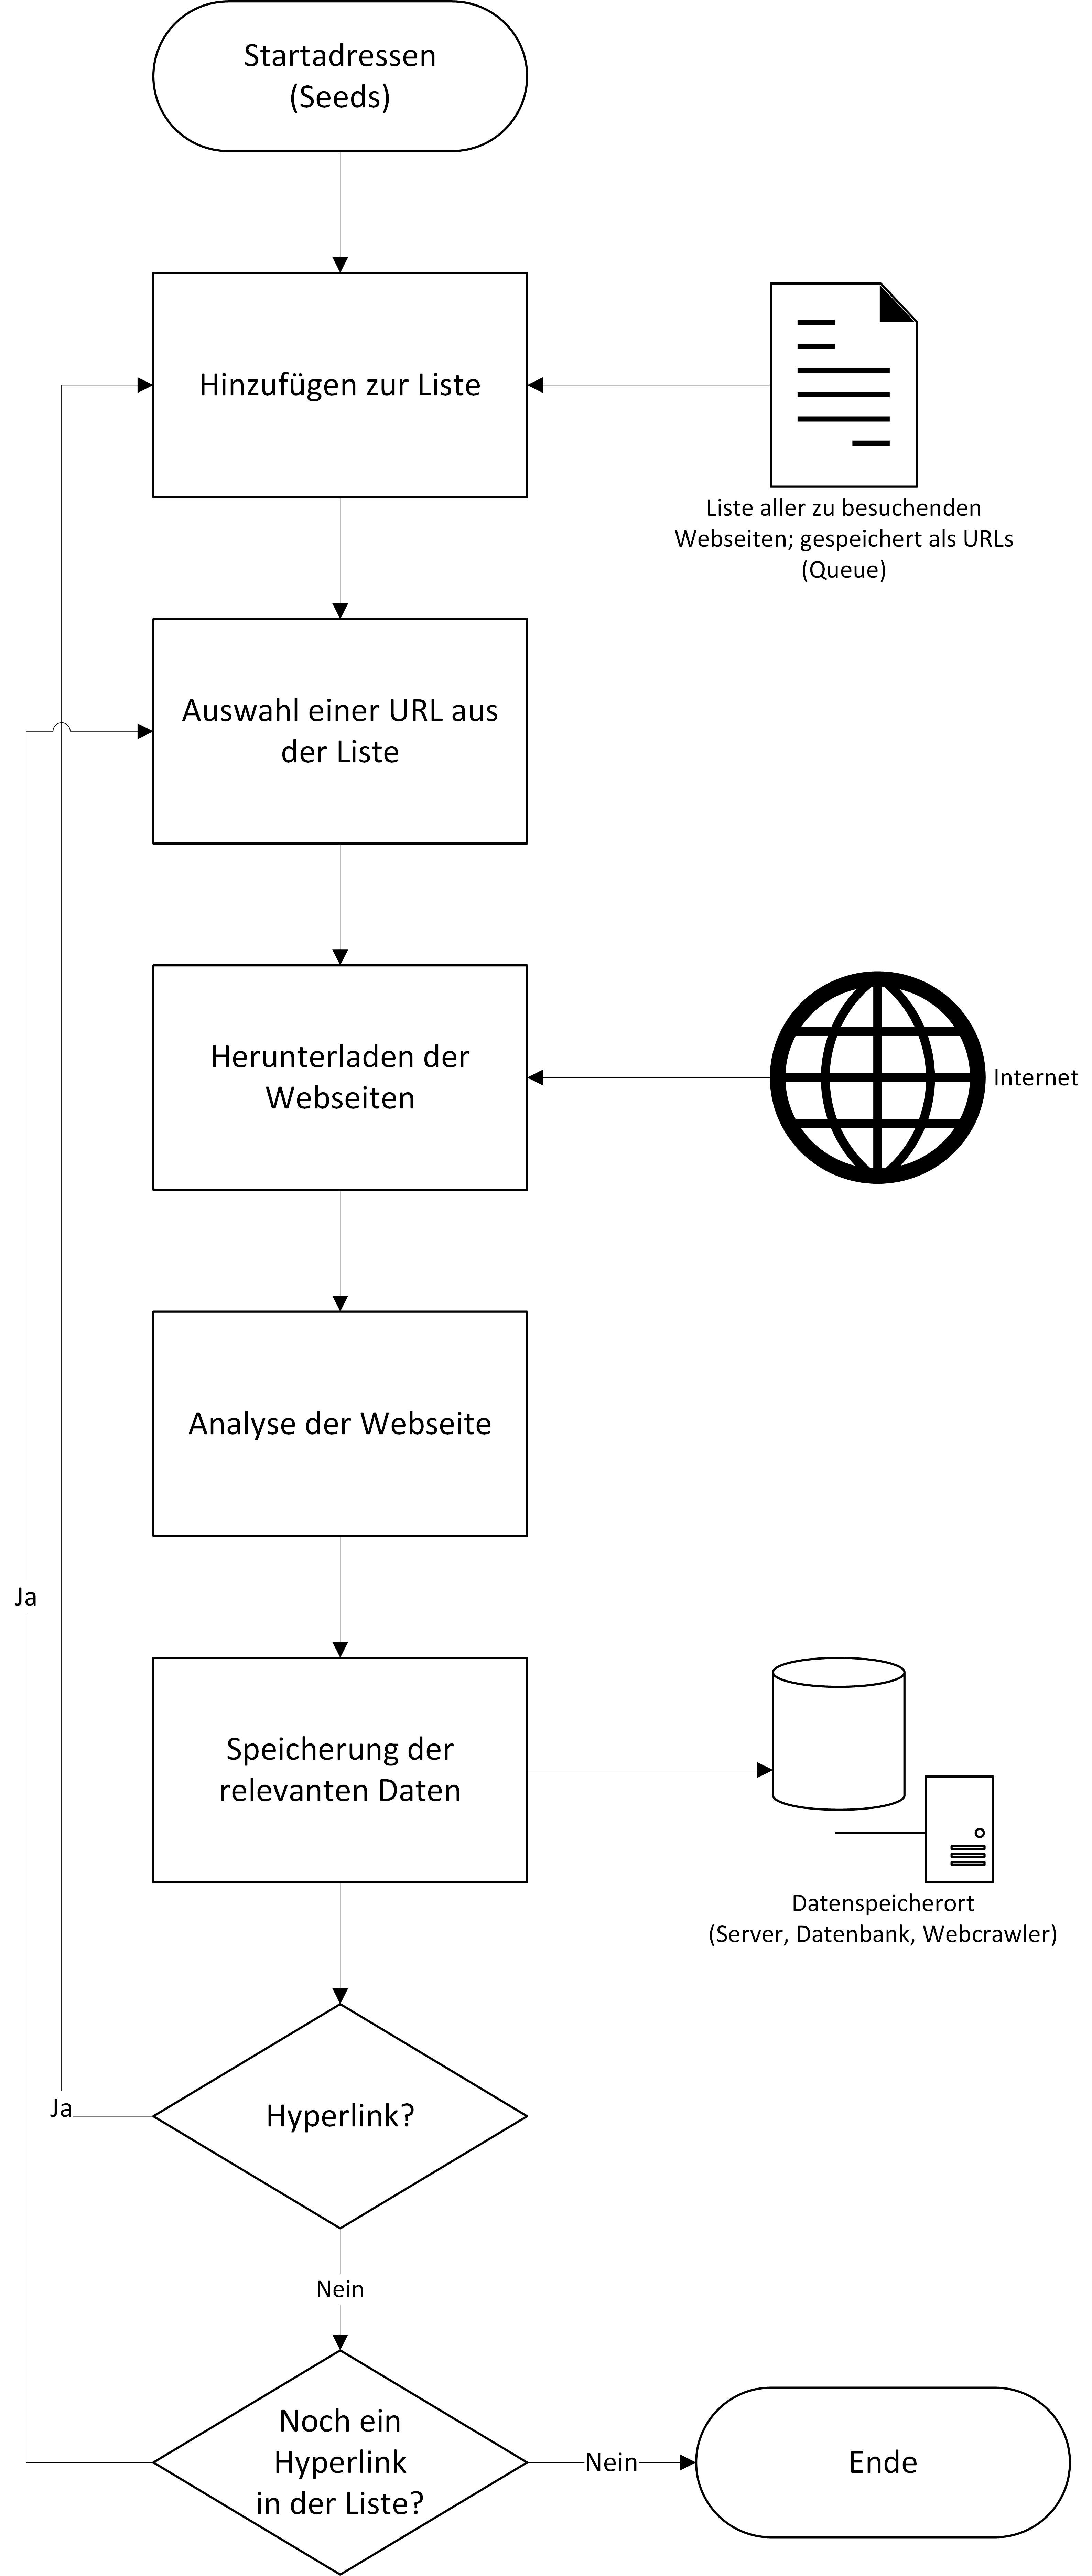
\includegraphics[width=8.45cm]{img/flussdiagramm-ablauf-webcrawler-neu.png}
	\caption{Arbeitsweise eines Webcrawlers}
	\label{fig:arbeitsweise_crawler}
\end{figure}
Da das Internet ein sich stets weiterentwickelndes und wandelndes Medium ist, in welchem sich Webseiten teils im Stundentakt ändern, muss ein Webcrawler gewissen Prinzipien folgen, welche in den folgenden vier Richtlinien aufgelistet sind.\cite[265-267]{ijcsc-web-crawler-overview} Somit kann gewährleistet werden, dass ein Webcrawler ein akzeptables Ergebnis erzielt.
\begin{enumerate}
	\item \textbf{Selection Policy \emph{(Auswahlrichtlinie)}}\newline
	Im Durchschnitt kommen alle zwei Sekunden rund zehn neue Webseiten hinzu\footnote{Messung selbst durchgeführt mit den Daten von internetlivestats.com\cite{zaehler-webseiten}.}. Dass ein Webcrawler nicht alle Webseiten besuchen kann ist somit selbsterklärend. Deshalb liegt es im Interesse des Betreibers eines Webcrawlers, dass dieser gezielt jene Webseiten untersucht, welche eine hohe Chance auf einen für den Betreiber relevanten Inhalt haben. Jeder unnötige Aufruf und jede unnötige Analyse einer Webseite verbraucht Ressourcen. Vor allem die Ressource \emph{Zeit} ist für Webcrawler  besonders wertvoll, denn mit jeder vergangenen Sekunde werden wieder neue Webseiten online gestellt. 
	%TODO: LÖSCHEN
	%Dies führt beispielsweise zu den unfassbaren 1.838.596.056 Webseiten\footcite[Stand Februar 2018:][]{stat-webseiten}, welche aktuell online sind.
	
	\item \textbf{Revisit Policy \emph{(Wiederbesuchsrichtlinie)}}\newline
	Neben den neu ins Netz gestellten Internetseiten, werden die bestehenden Webseiten auch stets aktualisiert. Neue Einträge kommen hinzu, alte werden gelöscht. Eines der besten Beispiele hierfür sind die unzähligen Nachrichtenportale im Internet: Dort werden oft im Minutentakt neue Meldungen, was im Grunde nichts anderes als neuer Inhalt ist, hinzugefügt. All dies sind Einträge, welche sich ein potentiell interessierter Webcrawler erneut holen und analysieren muss. Deshalb müssen Webcrawler abwägen, ob, wann und wie oft sie eine Seite erneut besuchen möchten oder auch müssen.
	%TODO: LÖSCHEN
	%, um ihren aktuellen \glqq Wissensstand\grqq\space auf einer der Webseite angemessenen Aktualität zu halten.
	
	\item \textbf{Politeness Policy \emph{(Höflichkeitsrichtlinie)}}\newline
	Eine Webseite ist heutzutage in wenigen Sekunden komplett geladen, Bilder, Videos oder ähnliche Medien inklusive. Bedenkt man nun, dass GoogleBot\footnote{Mehr zu GoogleBot in Kapitel \ref{subsub:googlebot}.}, ein Webcrawler des Internetgiganten Google, an die zehn Webseiten pro Sekunde\cite{googlebot-anzahl-pro-sekunde} anfragt und man mit einer durchschnittlichen Seitengröße von 3 Megabyte\cite{durch-seitengroesse} rechnen kann, so kommt man auf folgende einfache Gleichung:
	\begin{align*}
		10\ \nicefrac{Webseiten}{Sekunde}\ *\ 60\ Sekunden\ &=\ 600\ \nicefrac{Webseiten}{Minute}\\
		600\ \nicefrac{Webseiten}{Minute}\ *\ 60\ Minuten\ &=\ 36.000\ \nicefrac{Webseiten}{Stunde}\\
		36.000\ \nicefrac{Webseiten}{Stunde}\ *\ 3\ \nicefrac{Megabyte}{Webseite}\ &=\ 108.000\ \nicefrac{Megabyte}{Stunde} 
	\end{align*}
	Wie man hier erkennen kann, ist ein Webcrawler in der Lage, in kürzester Zeit eine Unmenge an Datenverkehr zu produzieren und somit wertvolle Bandbreite eines Webservers zu verschwenden. Da die Performance einer Webseite zu einem großen Teil auch von der Antwortzeit und der Auslastung des Webservers abhängt, kann durch einen Missbrauch eines Webcrawlers die Performance einer Webseite stark leiden. Während Webcrawler mit einem guten Zweck versuchen die Ressourcen des Webservers so wenig wie möglich in Anspruch zu nehmen, sind schadhafte, oder einfach nur schlecht geschriebene Webcrawler in der Lage ganze Server lahm zu legen und somit einen großen Schaden anzurichten.
	\item \textbf{Parallelization Policy \emph{(Parallelisierungsrichtlinie)}}\newline
	Da ein Webcrawler unter Umständen eine große Zeitspanne damit beschäftigt ist, auf die Antwort des Webservers zu warten, ist es natürlich selbstverständlich, dass man versucht die einem zur Verfügung stehenden Ressourcen bestmöglich auszunutzen. Ein Ansatz hierfür ist es, einen Webcrawler parallel ablaufen zu lassen. Hierfür müssen sich diese jedoch untereinander absprechen, damit zwei parallelisierte Webcrawler nicht dieselbe Webseite analysieren und somit erneut wertvolle Ressourcen verschwenden.
\end{enumerate}
Das Ziel eines jeden Entwicklers und Betreibers von Webcrawlern sollte es sein, diese vier Richtlinien zu respektieren und zu gewährleisten.\\
Diese Richtlinien werden jedoch des öfteren verletzt. Unerfahrene Programmierer können durch Programmierfehler diese Richtlinien unbewusst missachten und damit einen großen Schaden anrichten. Meistens werden diese Richtlinien jedoch bewusst verletzt, um in möglichst kurzer Zeit eine große Anzahl an Informationen zu gewinnen. Webcrawler, die diese Richtlinien bewusst verletzen, haben meist böse Absichten und sollten von den Webseiten ferngehalten werden.
\label{subsub:funk}








%\begin{figure}
%	\centering
%	\includegraphics[width=6cm]{flower}
%	\caption{Ein Beispiel.}
%	\label{fig:flower}
%\end{figure}







	%---Interaktion---
	\subsubsection{Interaktionsmöglichkeiten}
Das Internet ist ein öffentliche Medium und somit sind auch die Webseiten für jedermann zugänglich. Diese Tatsache hat maßgeblich zur Beliebtheit und zum Erfolg des Internets beigetragen und genau deshalb setzen so viele Unternehmen auf das Internet als Werbefläche. Haben Webseitenbetreiber also überhaupt eine Möglichkeit bösartige oder unerwünschte Webcrawler von ihren Webseiten fernzuhalten? In den vergangen Jahren wurden jedenfalls vermehrt Mittel geschaffen, um Betreibern von Webseiten die Möglichkeit zu geben mit Webcrawlern zu interagieren. Auf die bekanntesten dieser Mittel soll nun kurz eingegangen werden.
\begin{description}
	\item[robots.txt]
	Das Robots Exclusion Protocol, besser bekannt als \emph{robots.txt} wurde 1994\cite{robots-date} vom Holländer Martijn Koster\cite{robots-martijn} erfunden und hat sich zum de-facto-Standard in Sachen Interaktion mit Webcrawlern entwickelt, obwohl es nie ein offizieller Standard wurde.\cite{robots-date}\\
Um das Robots Exclusion Protocol zu verwenden, muss eine Datei mit dem Namen \emph{robots.txt} im Wurzelverzeichnis der Webseite abgespeichert werden. In dieser Datei können dann Regeln festgelegt werden, die besagen, welcher Webcrawler welche Dateien und Ordner besuchen darf bzw. welche nicht. Das einhalten dieser Regeln ist jedoch fakultativ, weshalb Webcrawler die Regeln der robots.txt auch einfach ignorieren können.
	\item[.htaccess]
	\emph{.htaccess} ist der Name einer Textdatei, die für die Konfiguration eines Apache Webservers verwendet wird. Da der Webserver von Apache die im Internet mit einem Marktanteil von 46,9\%\cite[Stand 24.03.2018:][]{statistik-webserver} am weitesten verbreitete Serversoftware ist, ist auch die Verbreitung von .htaccess dementsprechend hoch.
%TODO LÖSCHEN
%Die .htaccess-Datei kann dabei an jeden x-beliebigen Ort innerhalb des Webservers platziert werden. Die Regeln sind dann für diesen Ordner und alle Unterordner wirksam\cite{htaccess}.
Apache akzeptiert hierbei eine Vielzahl an Regeln in der .htaccess-Datei; darunter auch Regeln, welche Anfragen anhand der IP-Adresse und/oder des User Agent\footnote{Ein \emph{User Agent} ist eine Zeichenfolge, welche bei jedem Aufruf einer Seite an den Webserver übermittelt wird. In ihr stehen verschiedenste Informationen zu verwendetem Browser, Betriebssystem etc.\cite{user-agent-info}.} blocken. Im Gegensatz zu robots.txt sind die Regeln in .htaccess verpflichtend.
	\item[<meta />]
	Der <meta />-Tag ist ein Tag im HTML-Header in welchem verschiedene Zusatzinformationen, wie Autor, Schlagwörter oder ähnliches dem aufrufenden Browser übermittelt werden können. Mit einer dieser Zusatzinformationen des <meta />-Tags kann der Betreiber einer Webseite auch mit den Webcrawlern von Suchmaschinenbetreibern interagieren. Mit dem Tag \emph{<meta name="robots" content="noindex, nofollow" />} kann der Betreiber beispielsweise den Anbietern von Suchmaschinen mitteilen, dass er diese HTML-Seite nicht in die möglichen Suchresultate aufnehmen möchte und der Webcrawler keinen weiteren Hyperlinks auf dieser Seite folgen sollte\cite{meta-w3c}.
Wie bei der Verwendung von robots.txt ist auch diese Einhaltung fakultativ.\cite{meta-beispiel}
	\item[Automated Content Access Protocol]
	Das \underline{A}utomated \underline{C}ontent \underline{A}ccess \underline{P}rotocol (kurz ACAP) ist ein 2007 gegründetes Projekt, welches die Copyright-Ansprüche von Inhaltserstellern im Internet besser schützen soll.\cite{acap-was} Es will hierbei das weitverbreitete robots.txt nicht verdrängen, sondern eine Alternative bieten. ACAP wird heutzutage kaum verwendet,  da es namhafte Internetkonzerne, wie etwa Google, nicht nutzen\cite{acap-google}.
	%TODO: löschen wenns nimma braucht
	%\item[Webserver spezifische Mittel]
	%Abhängig von der gewählten Webserversoftware sind verschiedene Plugins, Module,  Erweiterungen, Optionen, usw. verfügbar mit denen sich der Zugriff regulieren lässt. Bwwährt hat sich die Devise: Je bekannter die Software, desto  mehr Plugins gibt es.
So ist das Modul \emph{mod\textunderscore authz\textunderscore host} beispielsweise eines der beliebtesten Module wenn es um Anfragebeschränkungen für den Apache Server geht\footcite{apache-module-beschraenkung}.
\end{description}

	%---GoogleBot---
	\subsubsection{GoogleBot}
Einer der wohl bekanntesten Webcrawler ist der \emph{GoogleBot}. GoogleBot ist der Webcrawler von Google, der größte Suchmaschinenanbieter weltweit mit über 90\% Marktanteil\cite{google-marktanteil}. Google setzt hierbei Algorithmen ein, um die GoogleBots zu steuern und festzulegen, welche Webseite wann und wie oft abgerufen wird\cite{googlebot-googleconsole}. Die gecrawlten Seiten werden dann von Google indexiert\footnote{Die Indexierung einer Webseite durch einen Suchmaschinenbetreiber bedeutet nichts anderes, als dass die Webseite von einem Suchmaschinenbetreiber gefunden wurde. Indexierte Webseiten werden dann in einem zweiten Moment als Vorschlag auf eine Suchanfrage ausgegeben.\cite{was-ist-indexieren}} und können im Bedarfsfall abgerufen und als Suchergebnisse in Bruchteilen einer Sekunde ausgegeben werden.\\
Da GoogleBot der weltweit größte operierende Webcrawler ist, ist er auch einer der am besten dokumentierten Webcrawler. Hier ein paar Fakten über den GoogleBot:
\begin{itemize}
	\item Im Jahre 2012 hatte Google mit seinem GoogleBot bereits 96\%\cite{googlebot-facts-percentage} aller Webseiten weltweit gecrawlt, Tendenz steigend. 
	\item Der User Agent von GoogleBot lautet\\\texttt{Mozilla/5.0 (compatible; Googlebot/2.1;\\+http://www.google.com/bot.html)}\cite{googlebot-user-agent}. 
	\item Im Durchschnitt besuchen GoogleBots eine Webseite 187mal am Tag\cite{googlebot-facts-incapsula}.\footnote{\label{footnote:incapsula-studie}Wert aus einer 2014 von Incapsula (amerikanisches Softwareunternehmen) durchgeführten Studie, in der sie 10.000 Webseiten ihrer Kunden über 30 Tage lang beobachteten.}
	\item Durchschnittlich stammt jeder fünfundzwanzigste Besuch von einem GoogleBot \emph{nicht} von GoogleBot. Dies bedeutet dass bösartige Bots den User Agent vom GoogleBot missbrauchen, um sich als dieser auszugeben und so unerkannt zu bleiben.\cite{googlebot-facts-incapsula}\textsuperscript{\ref{footnote:incapsula-studie}}
	\item Google verwendet mehrere Crawler, welche für unterschiedliche Zwecke entworfen wurden\cite{googlebot-user-agent}.
\end{itemize}
\label{subsub:googlebot}


	%--------------------------------
	%---Tarpiting---
	\subsection{Tarpitting}
	%---Definition---
	\subsubsection{Definition}
Unter Tarpitting versteht man den Vorgang, bei welchem ein Webcrawler mithilfe einer Tarpit durch verschiedenste Maßnahmen angelockt und später ausgebremst bzw. ausgeschaltet wird. Tarpits können dabei auf allen Layern des ISO/OSI-Modells\footnote{Das ISO/OSI-Modell ist ein Schichtenmodell, welches heutzutage das theoretische Modell für die Datenkommunikation zwischen Computern in einem Netzwerk und im Internet bildet\cite[430]{gallenbacher-iso-osi}.} implementiert werden\cite{tarpit-wikipedia}. Das Prinzip einer Tarpit ist dabei analog zu ihrem Namensgeber, einer Teergrube (engl. Tarpit), in welcher beispielsweise Tiere steckenbleiben. Tarpits arbeiten heutzutage oft in Kombination mit einem Honeypot\footnote{Ein \emph{Honeybot} ist ein System, welches versucht, Angreifer anzulocken, mit dem Ziel, Informationen wie die IP-Adresse oder den Standpunkt dieser herauszufinden oder neue Angriffsmethoden zu erkennen. Hierbei ist ein Honeypot ein \glqq normales\grqq\space System, welches jedoch bewusst bekannte Sicherheitsschwachstellen und -lücken aufweist\cite{def-honeybot}.}, welcher die Bots anlocken soll. Die Ausdrücke Honeypot und Tarpit werden deshalb heutzutage oft als Synonym verwendet\cite{honeypot-tarpit-synonym}.
Da tarpitting ein Mittel zur Bekämpfung von Bots ist, wird versucht es weitestgehend geheim zuhalten um den Entwicklern von Bots keine möglichen Schwachstellen aufzuzeigen. Deshalb ist, wenn überhaupt, nur eine unvollständige Dokumentation öffentlich einsehbar. Auch die IP-Adressen und URLs von Tarpits werden geheimgehalten.
\label{subsub:tarpitting}
	%---Formen---
	\subsubsection{Formen}
Wie bereits erwähnt, können Tarpits theoretisch in jedem Layer des ISO/OSI-Modells implementiert werden. Doch vor allem die Implementation und der Betrieb auf den unteren Schichten des ISO/OSI-Modells ist aufwendig, mühsam und fehleranfällig, da es dort keine Mittel zur Identifikation der Pakete und Einteilung derselbigen in \glqq Gut\grqq\space und \glqq Böse\grqq\space gibt. Deshalb werden heutzutage Tarpits hauptsächlich im IP-, TCP- und Application-Layer eingesetzt.\\
Während Tarpits auf dem IP-Layer versuchen durch minimieren der versendeten Daten die Verbindung künstlich in die Länge zu ziehen, nutzen TCP-Tarpits den Three-Way-Handshake\footnote{Der Three-Way-Handshake wird vom Transmission Control Protocol (TCP) verwendet um eine Verbindung aufzubauen.} aus, um potentielle Angreifer in die Irre zu führen. Tarpits auf dem Application-Layer, lassen sich in zwei große Gruppen unterteilen: SMTP-Tarpits und HTTP-Tarpits. SMTP-Tarpits behindern Mailserver, welche unerwünschte E-Mails, vielfach als Spam bezeichnet, versenden, in dem sie beispielsweise den Verbindungsaufbau, welcher vor dem versenden stattfinden muss, verlangsamen\cite{tarpit-smtp}. Die Funktionsweise von HTTP-Tarpits wird im folgenden Abschnitt \ref{subsub:http-tarpit} genauer beschrieben.

	%---HTTP---
	\subsubsection{HTTP-Tarpit}
HTTP-Tarpits sind neben SMTP-Tarpits eine der am häufigsten eingesetzten Tarpits. Sie haben aber weniger das Ziel den Gegenüber auszubremsen, sondern ihn eine möglichst lange Zeit zu \glqq beschäftigen\grqq , indem sie ihm stets neue unsinnige Informationen liefern.\\
Wie aus Abbildung \ref{fig:arbeitsweise_crawler}, Abschnitt \ref{subsub:funk}, erkennbar ist, besitzen Webcrawler eine Queue, in welcher die Adressen aller noch zu besuchenden Webseiten vermerkt sind. Ziel einer HTTP-Tarpit ist es nun, diese Queue kontinuierlich mit sinnlosen Adressen zu befüllen, damit ein gefangener Webcrawler möglichst viel Zeit damit verbringt, diese Adressen zu besuchen. Die aufgebrachte Zeit ist für den Webcrawler verschwendete Zeit. Wie bereits vorhin erwähnt ist Zeit jedoch eine der wichtigsten Ressourcen eines Webcrawlers. Meist zeigen die generierten Adressen auf die Tarpit selber und somit beginnt der Prozess von neuem. Ausgereifte Tarpits sind hierbei in der Lage Webcrawler für mehrere Tage zu beschäftigen.\cite{tarpitting-http-linux-mag}\\
Eine HTTP-Tarpit ist auch in der Lage Harvester in ihrer Arbeit zu behindern. Hierzu werden einige der generierten Adressen durch E-Mail-Adressen ausgetauscht. Um die E-Mail-Adressen für den Harvester sichtbar zu machen, muss im HTML-Quelltext beim Hyperlinktag \emph{<a>} bei der Zieladresse der entsprechende Präfix \emph{mailto:} gesetzt werden. Der Tag sieht dann folgendermaßen aus: \emph{<a href:"mailto:jemand@example.com">jemand@example.com<a/>}.\\
Diese verbreiteten E-Mail-Adressen sind entweder \glqq tot\grqq, sprich sie führen zu keinem E-Mail-Server oder \glqq infiziert\grqq, sprich sie zeigen auf einen präparierten E-Mail-Server der beispielsweise SMTP-Tarpitting betreibt.\\
Obwohl die Dokumentation solcher Tarpits bewusst geheim gehalten wird, rüsten Entwickler von Webcrawlern ihre Programme kontinuierlich gegen solche Fallen. Sie limitieren beispielsweise die Anzahl der auf einer Domaine aufgerufenen Seiten oder bauen andere Abwehrmaßnahmen gegen Tarpits ein.\\
Zu bedenken ist auch, dass der Besitzer einer Tarpit hier absichtlich Ressourcen verschwendet, indem er bewusst bösartige Webcrawler auf dem Webserver hält. Mit jedem neuen Webcrawler steigt des Weiteren die Gefahr eines Denial of Service, sprich ein Zusammenbruch des Servers aufgrund von Überlastung, drastisch.\cite{tarpitting-http-eggendorf-auugn}\\
Auch ist die Frage nach der Legalität nicht vollständig geklärt. Rechtlich bewegt man sich mit dem Betreiben einer Tarpit in einer Grauzone. Um jedoch sich selbst abzusichern, sollte man mithilfe von robots.txt\footnote{Mehr zum Thema \emph{robots.txt} ist im Kapitel \ref{subsub:funk} auf Seite \pageref{subsub:funk} aufgezeigt.} die Webcrawler \glqq warnen\grqq , indem man sie ausschließt. Sollten Webcrawler dann trotzdem in die Tarpit geraten wurden sie vorher gewarnt und sind demnach \glqq selbst schuld\grqq\ \cite{honeypot-tarpit-synonym}. Somit ist auch gewährleistet, dass keine gutwilligen Webcrawler, wie etwa GoogleBot\footnote{Der Webcrawler GoogleBot wird in Kapitel \ref{subsub:googlebot} auf Seite  \pageref{subsub:googlebot} genauer beschrieben.}, welche sich an die Regeln von robots.txt halten, von der Tarpit betroffen sind\cite{tarpitting-http-eggendorf-auugn}.
\label{subsub:http-tarpit}
	%##########################################
	%---Hauptteil---
	\section{Hauptteil}
	%---Ziel---
	\subsection{Ziel des Projektes}
	Ziel dieses Projektes ist, die vorher eingeführten Konzepte der Webcrawler mithilfe verschiedenster Arten von HTTP-Tarpits zu beweisen. Hierbei werden, wie unter Punkt \ref{umsetzung_grundlegendes} beschrieben, drei verschiedene Formen einer HTTP-Tarpit umgesetzt. Webcrawler sollen dann in diese Tarpit geraten. Ihr Verhalten innerhalb dieser Tarpit wird dann mitgeloggt und anschließend mithilfe von Drittanbietersoftware auf crawlertypische Verhaltensmuster hin analysiert. Des Weiteren wird der Zusammenhang zwischen Webcrawlern und allgemein bekannten Gefahren bei der Benutzung des Internets, wie beispielsweise das Veröffentlichen der E-Mail-Adresse auf einer Webseite oder das Benutzen von schwachen Passwörtern, untersucht und die Risiken und Auswirkungen dieser Gefahren aufgezeigt.
	%---Umsetzung---
	%TODO: BESSEREN NAMEN
	\subsection{Umsetzung}
	%---Grundlegendes---
	\subsubsection{Allgemein}
Um Webcrawler analysieren zu können wurde eine kleine Webseite erstellt und auf einem Raspberry Pi\footnote{Ein Raspberry Pi ist ein sogenannter Einplatinencomputer, sprich ein Computer dessen gesamte Komponenten auf einer einzigen Platine zusammengelötet wurden. Ein Raspberry Pi zeichnet sich durch ein ausgezeichnetes Preis/Leistungsverhältnis mit einer für die meisten Anforderungen ausreichende Leistung bei einem moderaten Preis von ca. 50\euro\space aus. Er wurde für den Dauerbetrieb entwickelt und eignet sich deshalb bestens für einen Webserver.} betrieben. Als Webserver wurde hierbei Apache verwendet, da es sich durch die weite Verbreitung und eine Vielzahl an hinzufügbaren Erweiterungen bestens eignet. Da sowohl Apache als auch dessen Erweiterungsmodule Open Source sind, sprich der Quelltext ist öffentlich zugänglich, stehen sie kostenlos zum Download bereit.\\
%TODO: evtl Linux als BS erwähnen
Die Webseite wurde größtenteils in PHP verfasst. PHP ist eine relativ alte, aber dennoch weit verbreitete Skript-Sprache mit der sich dynamische Webseiten generieren lassen.\\
Die Webseite trägt den Namen \emph{VEVETA} und ist öffentlich unter der Adresse \url{http://maturaprojekt.ddns.net} erreichbar. \emph{VEVETA} steht hierbei für \underline{VE}rbund \underline{VE}rschiedener \underline{TA}rpits und vermittelt somit sofort den Zweck dieser Webseite: Drei verschiedene Tarpitformen werden implementiert, um gleichzeitig drei verschiedene Arten von Webcrawlern anlocken und fangen zu können:
\begin{description}
	\item[Hyperlink-Tarpit] Hierbei werden verschiedene Hyperlinks, wie unter Punkt \ref{subsub:hyperlink-tarpit} beschrieben, ausgegeben, um somit jegliche Art von Webcrawlern anzulocken.
	\item[Harvester-Tarpit] Hierbei werden verschiedene zufällig generierte\\E-Mail-Adressen ausgegeben um Harvester anzulocken. Nähere Details hierzu sind unter Punkt \ref{subsub:harverster-tarpit} aufgeführt.
	\item[Brute-Force-Tarpit] Hier wird dem Aufrufer eine Log-In-Maske dargestellt. Jede Eingabe wird hierbei als \glqq falsch\grqq\space gewertet und mitgeloggt. Einzelheiten dazu sind unter Punkt \ref{subsub:brufe-force-tarpit} einsehbar.
\end{description}
Um den Verlauf der Tarpit besser beobachten zu können wurden kontinuierlich Logfiles\footnote{Ein Logfile ist eine Datei in der eine Software, je nach Konfiguration, verschiedene Informationen, speichert, um diese zu einem späteren Zeitpunkt auswerten zu können. Somit können Rückschlüsse auf Fehler, Auslastung und der gleichen gezogen werden.} geschrieben. Apache schreibt hierbei eigenständig einen Accesslog in welchem jeder Aufruf der Webseite mit IP-Adresse, Zeit, Adresse der aufgerufenen Seite, Referring Site\footnote{Eine Referring Site ist eine Webseite welche vor dem Aufruf der eigentlichen Webseite aufgerufen wurde, sprich es ist diese Webseite von der aus ein Aufrufer über einen Link auf eine andere, \glqq meine\grqq, Webseite gelangt ist.} und User-Agent notiert wird. Um diese Logfile kontinuierlich auswerten zu können, wurde die Open Source Drittanbieter-Software \emph{GoAcces\footnote{Nähere Informationen, Downloadlinks, Live-Demo, Dokumentation, etc. sind auf der \href{https://goaccess.io/}{\emph{Homepage}} von GoAccess angeführt.}} verwendet, welche Accesslogs auswertet und, unter anderem live, Statistiken über den Traffic\footnote{Als \emph{Traffic} einer Webseite bezeichnet man den anfallenden Datenverkehr, welcher beispielsweise durch einen Aufruf einer Seite entsteht.} der Webseite ausgibt.\\
Um alle Webcrawler vor den Gefahren zu warnen, muss die Datei robots.txt um die folgenden Zeilen entsprechend angepasst werden.
\begin{lstlisting}
	User-agent: *
		Disallow: /
\end{lstlisting}
Hiermit wird allen Webcrawlern empfohlen, die komplette Webseite zu meiden.
\label{umsetzung_grundlegendes}
	%---Hyperlink-Tarpit---
	\subsubsection{Hyperlink-Tarpit}
Die erste der drei implementierten Tarpitformen ist die klassische HTTP-Tarpit, wie sie auch unter Punkt \ref{subsub:http-tarpit} beschrieben ist. Hierbei werden fortlaufend neue Hyperlinks generiert, welche allesamt \glqq ins Leere\grqq,\space sprich auf keine weitere Webseite, zeigen. Dies würde bei einem herkömmlichen Webserver einen \emph{404 Not Found} HTTP-Statuscode hervorrufen, welcher dem Aufrufer mitteilt, dass die angeforderte Ressource, sprich die Webseite, auf dem Webserver nicht existiert. Ein vermehrtes auftreten von solchen 404-Codes würde einen Webcrawler alarmieren und er würde den Crawl-Vorgang abbrechen, da er der Meinung ist, auf diesem Webserver gäbe es nichts zu holen. Um dies zu verhindern muss dem Webserver mitgeteilt werden, dass wir bei einem 404-Code gerne eine eigene Seite anzeigen möchten. Dies kann bei Apache durch den Befehl
\begin{lstlisting}
ErrorDocument 404 [ADRESSE]
\end{lstlisting} 
erledigt werden. Diesen Befehl kann man dann sowohl in der Datei \emph{.htaccess} festlegen als auch in der Datei \emph{000-default.conf}, welche sich in Linux-Systemen unter dem Pfad \emph{/etc/apache2/sites-available/000-default.conf} befindet. Bei der Änderung der .conf-Datei ist jedoch Vorsicht geboten und es empfiehlt sich vorher ein Backup zu machen. Für den weiteren Verlauf dieses Projektes sollen alle 404-Codes auf die Datei \emph{reply.php} umgeleitet werden:
\begin{lstlisting}
ErrorDocument 404 /reply.php
\end{lstlisting}
Das PHP-Skript, welches in der Datei \emph{reply.php} enhalten ist, generiert dann eine Webseite mit zufälligem Text, welcher wiederum zufällige Hyperlinks enthält. Als aller erstes muss jedoch der 404-Statuscode vom Webserver unterbunden werden. Denn der zuvor aufgeführte Code leitet nur die Anfrage an die Datei reply.php weiter, behält jedoch den Statuscode, in diesem Fall 404, bei. Um den Statuscode zu ändern muss das PHP-Skript den Statuscode überschreiben und dem Aufrufer den HTTP-Statuscode \emph{200 OK} senden. Dies passiert in den folgenden Zeilen, welche am Beginn des PHP-Skriptes stehen und den HTTP-Header manipulieren:
\lstinputlisting[language=PHP, firstline=1, lastline=10]{sourcefiles/reply.php}
Da sich der Inhalt der durch das Skript generierten Webseite bei jedem Aufruf ändert, darf es nicht im Cache gespeichert werden.\footnote{Moderne Browser speichern, man spricht hier von cachen, Dateien für einen gewissen Zeitraum, damit sie bei einer erneuten Anfrage nicht erneut vom Webserver heruntergeladen werden müssen und somit Zeit und Traffic gespart wird.} Das Cachen der Webseite ist in diesem Fall schlecht, da es einen Webcrawler am Generieren von neuem Inhalt hindern könnte. Dies wird ebenfalls durch den zuvor aufgeführten Codeteil gewährleistet, da er sowohl das Änderungs-, als auch das Verfallsdatum für die Speicherung im Cache auf das aktuelle Datum setzt. Diese Zeitangaben muss in der Greenwich Mean Time\footnote{Die Greenwich Mean Time (GMT) ist die Zeitzone, welche in Greenwich/London gilt.} angegeben werden.\cite{http-header-time} Des Weiteren schreibt er ein \emph{no-store}, \emph{no-cache} und \emph{must-revalidate} vor, welche allesamt dem Aufrufer das Cachen der Webseite untersagt.\\
Das Skript generiert anschließend eine Webseite, welche aus drei unterschiedlich langen Spalten besteht. Die Spalten werden anschließend mit Buchstaben, Wörtern und Zeichen befüllt. Die Verteilung der Buchstaben entspricht dabei ungefähr den realen Werten der englischen Sprache. Hierfür wurde ein Array erstellt, in welchem die Buchstabe anhand der Verteilung der Buchstaben in der englischen Sprache aufgelistet sind.\footnote{Eine Tabelle der Verteilung der Buchstaben kann unter \url{http://kryptografie.de/kryptografie/kryptoanalyse/haeufigkeitsverteilung.htm} eingesehen werden.}
 Dies bedeutet, wenn ein Buchstabe beispielsweise eine sechs-prozentige Verteilung in der englischen Sprache aufweist, so belegt er auch sechs Prozent der verfügbaren Arrayplätze. Um die generierte Webseite noch realistischer wirken zu lassen und somit keinen Anschein einer Tarpit zu erwecken, wurden folgende Konzepte umgesetzt:
\begin{description}
	\item[Generieren von \grqq echten\grqq\space Wörter] Es werden neben den zufällig generierten Buchstaben auch noch vordefinierte englische Wörter\footnote{Beispiele für vordefinierte englische Wörter wären \emph{the}, \emph{be}, \emph{and} usw..}, Satzzeichen und Leerzeichen mit unterschiedlicher Wahrscheinlichkeit zum Text hinzugefügt. Durch das Einfügen von Leerzeichen entstehen weitere \grqq wörterähnliche\grqq\space Strukturen.
	\item[Variieren der Spaltenlänge] Die generierte Webseite besitzt drei Spalten, welche jeweils eine unterschiedliche Länge aufweisen. Eine Längeneinheit ist hierbei ein Zeichen oder ein vordefiniertes Wort. Die Länge der Spalten bewegt sich hierbei zwischen 3.000 und 4.000 Zeichen bzw. vordefinierte Wörter.
	\item[Generieren von Hyperlinks] Auf einer Webseite befinden sich durchschnittlich 6,4 Hyperlinks, welche auf einen anderen Bereich der Seite, eine komplett andere Webseite oder auf eine andere Domain zeigen.\cite{tarpitting-http-linux-mag} Je mehr Hyperlinks auf einer Webseite sind, umso effizienter kann man einen Webcrawler für eine Zeit lang \glqq beschäftigen\grqq . Damit die generierte Webseite jedoch trotzdem eine realistische Anzahl an Hyperlinks aufweist, generiert das PHP-Skript mit einer Wahrscheinlichkeit von einem Prozent eine Hyperlink auf einem zufällig generierten Ziel mit einer Länge zwischen 5 und 25 Zeichen. Dies ergibt bei einer Spaltenlänge von 3.000 bis 4.000 Zeichen eine durchschnittliche Hyperlink-Anzahl von 90 bis 120. Um die Struktur der Hyperlinks zu variieren zeigen sie jeweils mit einer Wahrscheinlichkeit von je 25\% auf eine Datei mit der Endung .htm oder .php und mit einer Wahrscheinlichkeit von 50\% auf eine .html-Datei. Die Verteilung dieser Wahrscheinlichkeiten ist nochmals in Abbildung \ref{fig:wahrbaum} auf Seite \pageref{fig:wahrbaum} aufgezeigt.
\end{description}
Somit generiert ein Webcrawler bei jedem Aufruf des Skriptes um die 100 neue Hyperlinks. Ruft er nun $n$-mal dieses Skript auf, so generiert er $100^n$ virtuelle, nicht existente, Dateien. Dies ist eine exponentielle Funktion, welche enorm schnell wächst. Bei sechs-maligem Aufrufen der Seite, was für einen Webcrawler de facto kein Aufwand ist, hat er somit bereits $100^6 = 1.000.000.000.000$ (Eine Billion) Hyperlinks gezeugt, welche in seiner Queue gespeichert sind. Wenn ein Webcrawler theoretisch ein Zehntel einer Sekunde für das Abarbeiten einer Webseite brauchen würde, wäre er hiermit schon über 31.000 Jahre beschäftigt.\\
Ein Webcrawler ist somit schnell gefangen. Sollte ein Webcrawler die Falle bemerken, so wurde zumindest seine Queue unbrauchbar gemacht. Durch ein leeren dieser Queue würde der Webcrawler zwar wieder diese sinnlosen Hyperlinks los werden, jedoch würde er auch alle anderen darin gespeicherten Hyperlinks verlieren.\\
Anzumerken ist jedoch, dass die oben angegebenen Zahlen nur einem theoretischen Wert entsprechen und das Skript in der Praxis mit einer Wahrscheinlichkeit von 10\% anstelle der \glqq normalen\grqq\space Hyperlinks eine E-Mail-Adresse geniert, siehe hierfür Punkt \ref{subsub:harverster-tarpit}.\\
\begin{figure}[H]
	\centering
	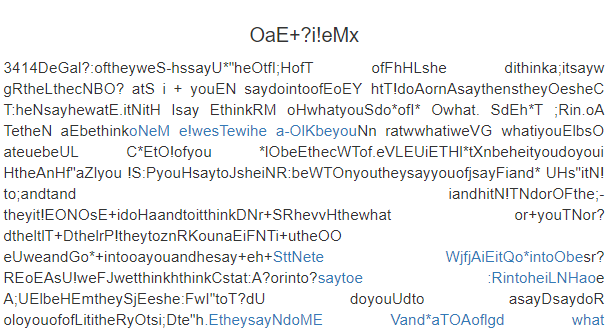
\includegraphics[width=8.45cm]{img/beispiel-hyperlink1.PNG}
	\caption{Beispielausgabe des Skriptes \emph{reply.php}. Zur besseren Übersicht wird nur eine der drei Spalten angezeigt}
	\label{fig:beispiel-hyperlink}
\end{figure}
Das gesamte reply.php-Skript ist in den Anhängen beigefügt und einsehbar.
\label{subsub:hyperlink-tarpit}


	%---Harvester-Tarpit---
	\subsubsection{Harvester-Tarpit}
Um Harvester in die Falle zu locken besitzt VEVETA zwei Methoden:
\begin{enumerate}
	\item Generieren einer E-Mail-Adresse anhand der IP-Adresse
	\item Generieren verschiedener E-Mail-Adressen
\end{enumerate}
\paragraph{Generieren einer E-Mail-Adresse anhand der IP-Adresse}\mbox{}\\
Dem Aufrufer wird auf der Landingpage\footnote{Als Landingpage wird in der Regel jene Webseite bezeichnet, welche beim Aufruf einer URL als erstes angezeigt wird} neben einem Kontaktformular eine E-Mail-Adresse angezeigt, welche folgende Form aufweist: \emph{[IP-ADRESSE]-[DATUM]-[UHRZEIT]@maturaprojekt.ddns.net}.\\
Damit Harvester diese E-Mail-Adresse auch schnell finden, wurde sie mit dem Schlüsselwort \emph{mailto:} gekennzeichnet, das in HTML als Kennzeichen für eine E-Mail-Adresse verwendet wird. Der Code zum generieren dieser E-Mail-Adresse ist in der Datei \emph{index.php} inkludiert:\\
\lstinputlisting[language=PHP, firstline=378, lastline=389]{sourcefiles/index.php}
Ein Aufruf der Datei index.php würde beispielsweise folgende E-Mail-Adresse generieren:
\emph{82.52.47.189-02.04.2018-16.20.58@maturaprojekt.ddns.net}, welche aus den Augen eines Harvesters folgende HTML-Struktur aufweist:\\
\lstinputlisting[language=HTML]{sourcefiles/generated-mail.html}
\paragraph{Generieren verschiedener E-Mail-Adressen}\mbox{}\\
Des Weiteren generiert das Skript \emph{reply.php}, wie unter Punkt \ref{subsub:hyperlink-tarpit} beschrieben, auch E-Mail-Adressen. Wie unter demselben Punkt erwähnt, besteht die ein-prozentige Chance, dass ein Hyperlink generiert wird. Wenn dieser Fall eintritt, besteht des Weiteren eine zehn-prozentige Chance, dass anstelle eines Hyperlinks eine E-Mail-Adresse generiert wird. Somit wird mit einer Wahrscheinlichkeit von 0,1\% eine E-Mail-Adresse vom Skript generiert. Dies entspricht in etwa fünf bis zehn E-Mail-Adressen pro generierter Webseite. Um diese E-Mail-Adressen so realistisch als möglich aussehen zu lassen, wurden online auf der Webseite \url{http://www.freedatagenerator.com/csv-data-generator} E-Mail-Adressen generiert, von denen eine mit einer Wahrscheinlichkeit 50\% ausgewählt wird; ansonsten wird eine E-Mail-Adresse bestehend aus zufälligen Zeichen generiert. Bei beiden Varianten wird vorne an der E-Mail-Adresse die Zeit zum Zeitpunkt des Generierens in Form eines Unix-Timestamps\footnote{Der Unix-Timestamp ist eine einfache, aber dennoch exakte Art Zeit zu messen. Der Unix-Timestamp besteht aus einer Zahl, welche die Anzahl an Sekunden, die seit dem 1. Januar 1970 vergangen sind, angibt.} angefügt.\\
Die Verteilung der Ausgabe des Skriptes reply.php ist in der Abbildung \ref{fig:wahrbaum} aufgeführt.\\
Alle E-Mail-Adressen verweisen auf die Domain \emph{@maturaprojekt.ddns.net} und landen somit auf einem Mail-Server, welcher neben dem Apache-Webserver auf dem Raspberry Pi läuft.\\
Diese Form der Tarpit dient in erster Linie dazu, Harvester zu entlarven und ihre Mailinglisten mit unsinnigen E-Mail-Adressen zu verstopfen. Durch das Anhängen des Timestamps kann man im Nachhinein herausfinden, welche IP-Adresse und welcher User-Agent zu einem Harvester gehörte, da man diese in den Logfiles beim Eintrag, dessen Zeit zum Timestamp korrespondiert, ablesen kann. Da der Timestamp jedoch erst nachträglich eingefügt wurde, können nicht mehr alle E-Mail-Adressen einem Harvester zugeordnet werden.
\begin{figure}[H]
	\centering
	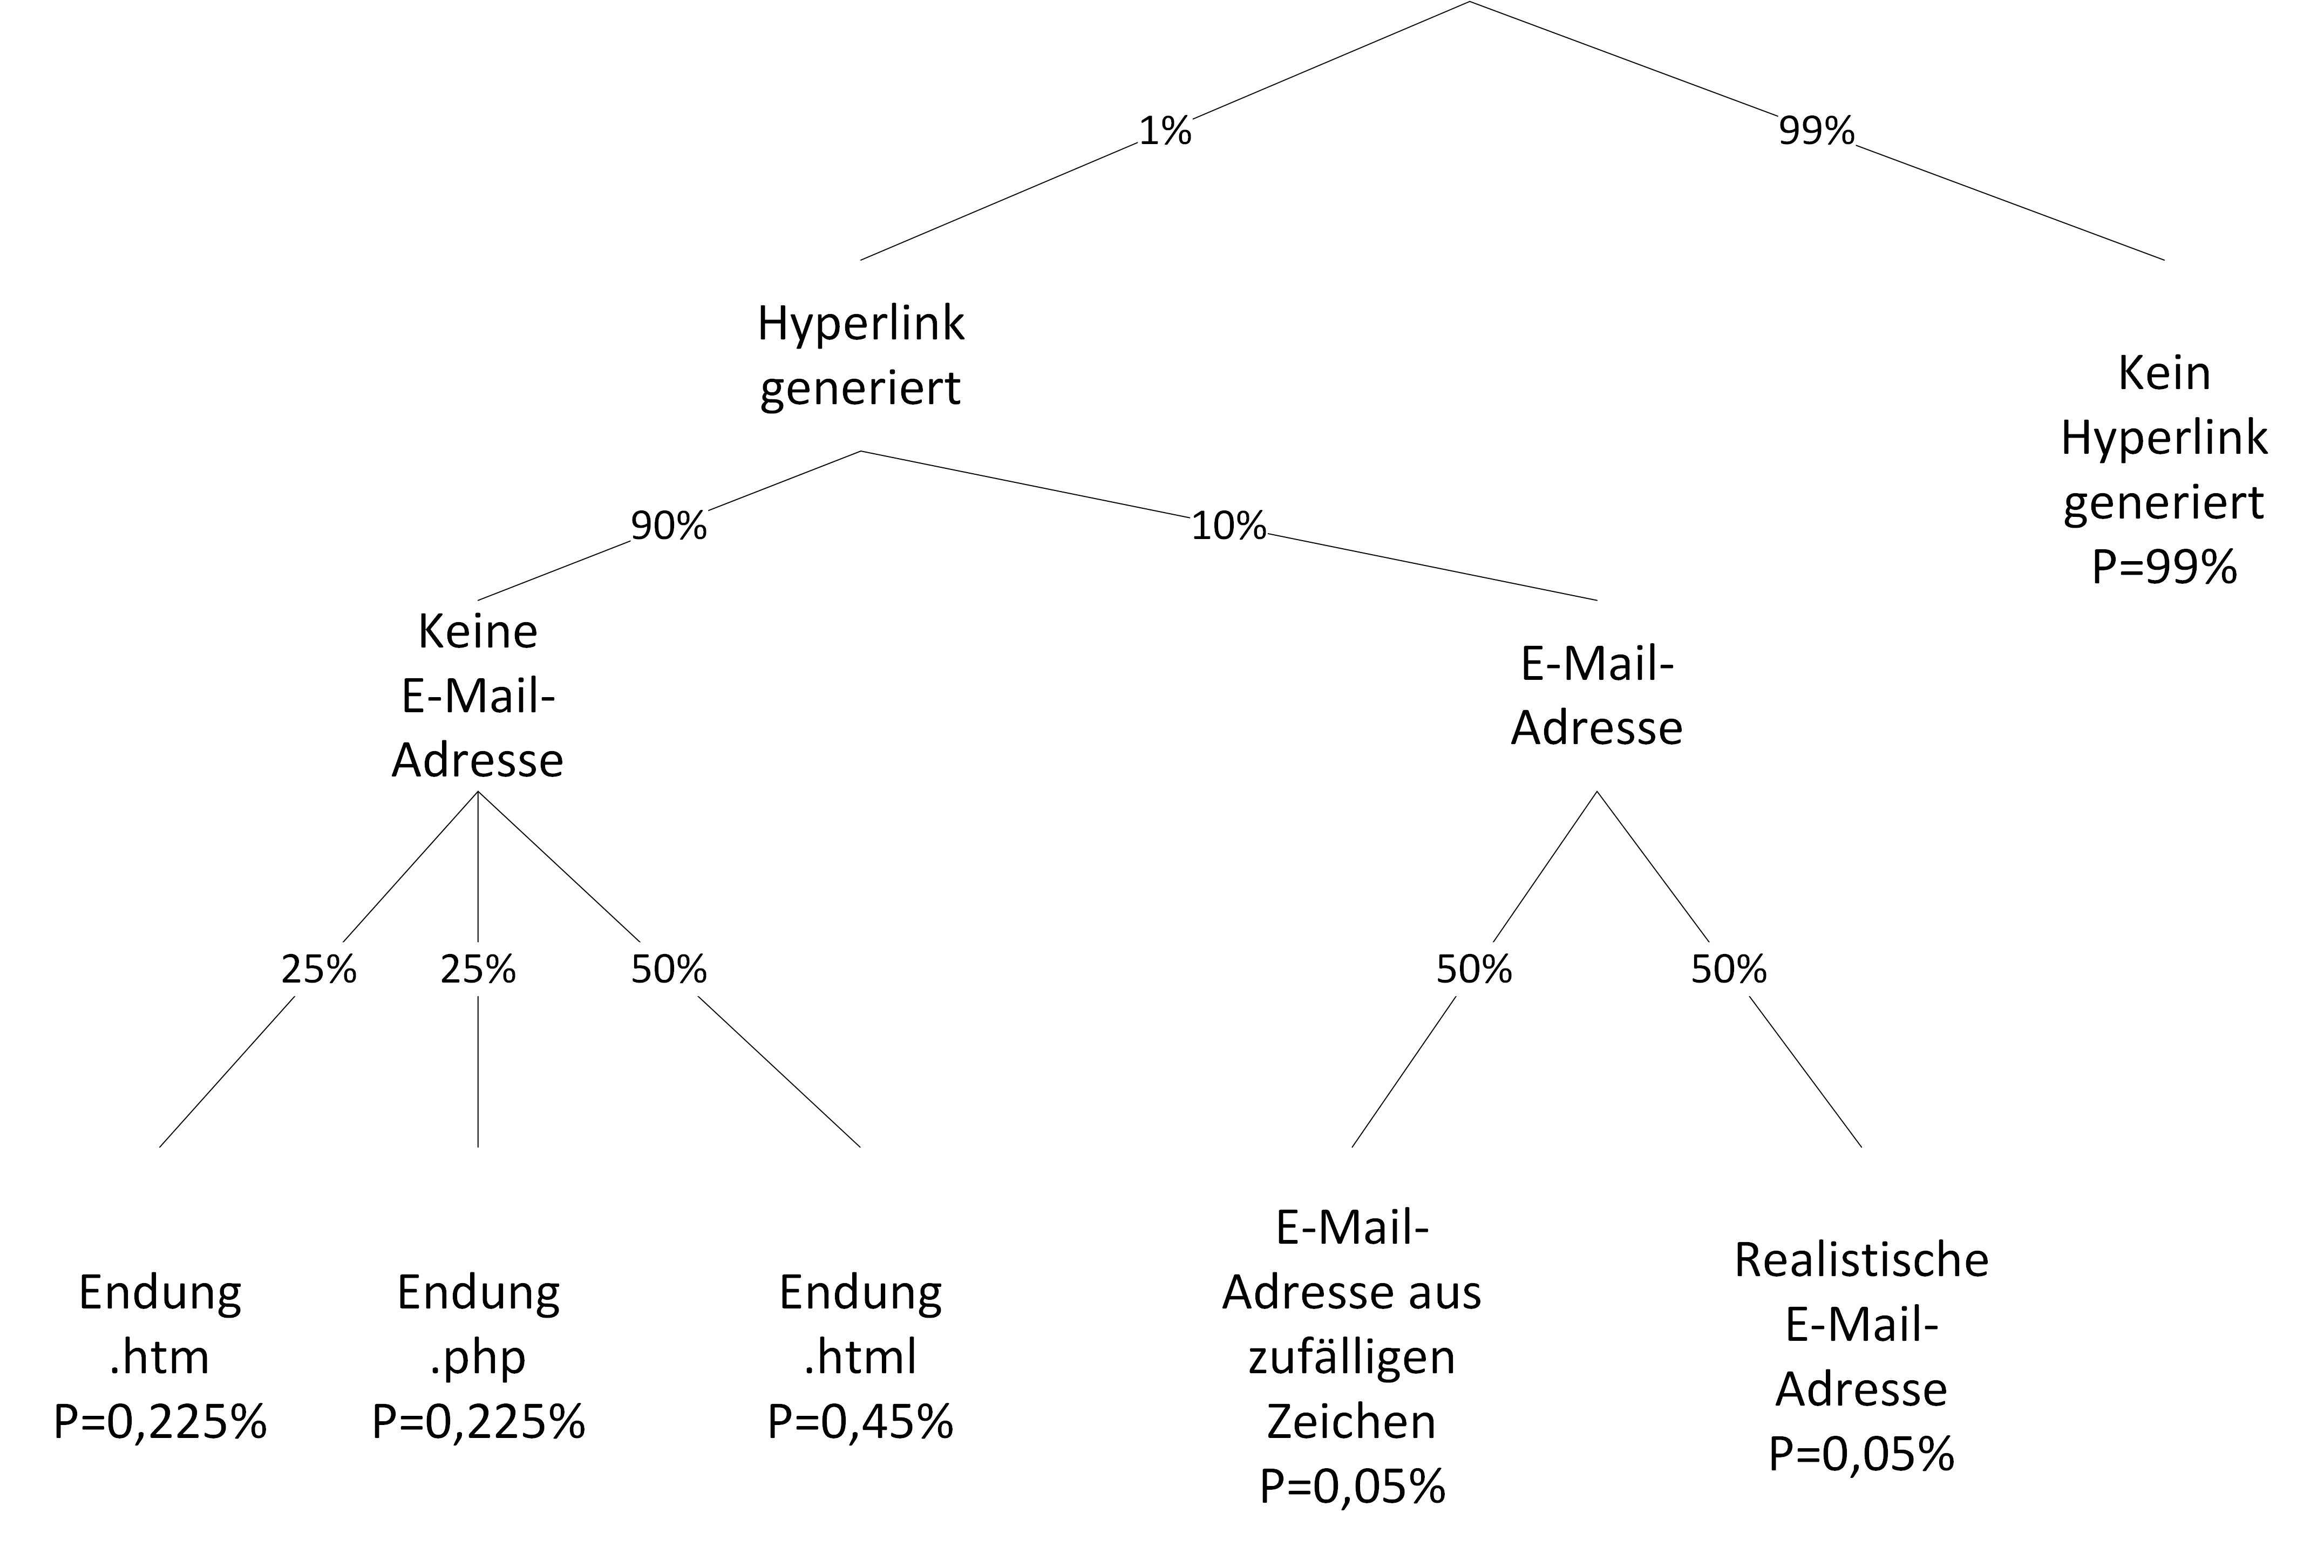
\includegraphics[width=8.45cm]{img/Wahrscheinlichkeitsbaum.png}
	\caption{Wahrscheinlichkeitsbaum der Ausgabe des Skriptes \emph{reply.php}. Die Wahrscheinlichkeit ist am jeweils letzten Blatt eines Astes angeführt. \emph{P} entspricht hier der Wahrscheinlichkeit}
	\label{fig:wahrbaum}
\end{figure}
%% The sloped option gives rotated edge labels. Personally
% I find sloped labels a bit difficult to read. Remove the sloped options
% to get horizontal labels. 
\begin{tikzpicture}[grow=down]
\node[bag] {}
    child {
        node[bag] {Hyperlink generiert}        
            child {
                node[bag] {E-Mail-Adresse}
                child {
                	node[end, label=below:
                	{E-Mail-Adresse aus zufällig generierten Zeichen}] {}
                	edge from parent
                	node[below]  {50\%}
                }
                child {
                	node[end, label=below:
                	{realistische E-Mail-Adresse}] {}
                	edge from parent
                	node[below]  {50\%}
                }
                edge from parent
                node[below]  {10\%}
            }
            child {
            	node[bag] {keine E-Mail-Adresse}
            	child {
            		node[end, label=below:
            		{Endung .htm}] {}
            		edge from parent
            		node[below]  {25\%}
            	}
	            child {
	            	node[end, label=below:
	            	{Endung .php}] {}
	            	edge from parent
	            	node[below]  {25\%}
	            }
            	child {
            		node[end, label=below:
            		{Endung .html}] {}
            		edge from parent
            		node[below]  {50\%}
            	}
            	edge from parent
            	node[below]  {90\%}
            }
            edge from parent 
            node[below]  {1\%}
    }
    child {
        node[end, label=below:
        {kein Hyperlink generiert}] {}
        edge from parent
        node[below]  {99\%}
    };
\end{tikzpicture}
\label{subsub:harverster-tarpit}

	%---Brute-Force-Tarpit---
	\subsubsection{Brute-Force-Tarpit}
Eine der gängigsten  Arten um Passwörter zu knacken ist die sogenannte \emph{Brute-Force}-Methode, zu Deutsch \glqq rohe Gewalt\grqq-Methode. Hierbei werden gängige Kombinationen aus Benutzername und Passwort in einem Anmeldeformular ausprobiert, mit der Hoffnung, dass eine der Kombinationen richtig ist.\\
Die erstellte Tarpit bietet auch eine Anlaufstelle für solche Webcrawler. Unter der URL \url{http://maturaprojekt.ddns.net/wp-login.php} ist ein WordPress-Login simuliert. WordPress ist mit 60\% Marktanteil\cite{wordpress-verbreitung} das am weiten Verbreiteste Content-Management-System\footnote{Ein Content-Management-System (CMS) ist eine Software, welche einen oder mehrere Anwender bei der Erstellung, Barbeitung und Verwaltung von Inhalten, meist Webseiten, unterstützt.} und erfreut sich großer Beliebtheit. Durch die einfache und schnelle Installation bzw. Einrichtung ist Wordpress auch bei Anfängern eine beliebte Software für das Erstellen einer Webseite. Um Änderungen an der Webseite vornehmen zu können, müssen sich die Anwender über eine Log-In-Form anmelden, welche standardmäßig über \emph{[DOMAINE]/wp-login.php} erreichbar ist. Durch die weite Verbreitung und den allgemein bekannten Standartpfad ist diese Log-In-Form ein häufiges Ziel von Brute-Force-Angriffen. Webcrawler überprüfen, ob sie die zuvor erwähnte Log-In-Form unter der gewohnten Adresse finden und starten dann mit einem Brute-Force-Angriff auf diese Log-In-Maske.\\
VEVETA besitzt ebenfalls eine WordPress-Log-In-Form. Die Struktur dieser stammt aus einer öffentlich zugänglichen Demo von \emph{Softaculous}\footnote{Die Demo ist Einsehbar unter der Adresse \url{https://demos1.softaculous.com/WordPress/wp-login.php}.}, welche so modifiziert wurde, dass sie den Anschein einer gängigen WordPress-Log-In-Form der Webseite \emph{maturaprojekt.ddns.net} erweckt. Die darin enthaltene Eingabeform ist so modifiziert, dass nach dem Absenden der Eingabedaten diese in einem Log zusammen mit IP-Adresse und Datum gespeichert werden. Der hier aufgezeigte Codeabschnitt ist für dies verantwortlich:
\lstinputlisting[language=PHP, firstline=21, lastline=31]{sourcefiles/wp-login.php}
Nach dem Abschicken der Log-In-Daten wird der Aufrufer wieder auf die Seite \emph{/wp-login.php} zurück geleitet, dies erzeugt den Eindruck eines falsch eingegebenen Passworts und der Aufrufer kann seine nächste Kombination aus Benutzername und Passwort ausprobieren. Diese Art der Tarpit dient somit in erster Linie der Analyse von Webcrawlern, welche die Absicht haben, Brute-Force-Angriffe auf einer Webseite auszuüben.
\label{subsub:brufe-force-tarpit}
	%---Auswertung---
	\subsection{Auswertung}
	%---Hyperlink-Tarpit---
	\subsubsection{Hyperlink-Tarpit}
Die erste der drei Tarpitformen, die VEVETA implementiert, ist, wie bereits zuvor erwähnt, die Hyperlink-Tarpit, dessen Ziel es ist, die Queue von klassischen Webcrawlern mit sinnlosen Hyperlinks zu verstopfen und sie so im besten Fall zu fangen. Hierbei lieferte die Analyse mit \emph{GoAccess} folgende Resultate\footnote{Die Resultate basieren auf den Logfiles, welche zwischen dem 01. August 2017 und 04. April 2018, sprich innerhalb von ca. acht Monaten, erstellt wurden.}:\\
In den 247 Tagen, in welchen die Tarpit online war, wurden 342.020 Anfragen von 20.232 verschiedenen Besuchern\footnote{GoAcces zählt alle Aufrufe, welche an einem Tag von der gleichen IP-Adresse aus mit dem gleichen User-Agent getätigt wurden, als einen Besucher.} gezählt, dies entspricht einem Mittel von 1.384,69 Anfragen pro Tag. Wenn man bedenkt, dass die Seite nur für das Fangen von Webcrawlern online gestellt wurde, ist dies ein akzeptabler Wert. Im Durchschnitt hat hierbei jeder Besucher 16,9 Anfragen getätigt. Es wurden hierbei 185.300 verschiedene Webseiten bzw. Dateien angefragt, einige davon natürlich auch mehrfach. Ein Logfile, in welchem der Name und das Datum der generierten virtuellen Dateien gespeichert wurde, hatte am 04. April über 28.510.000 Einträge. Das Skript in reply.php zeigte somit sein volles Potential.
\begin{table}[htb!]
	\centering
	\begin{tabular}{c|r}
		\textbf{Anzahl der Anfragen}&\textbf{Datum}\\\hline
		17.687&20. Dezember 2017\\
		17.117&22. Dezember 2017\\
		16.925&21. Dezember 2017\\
		16.853&19. Dezember 2017\\
		15.299&24. Dezember 2017\\
		15.076&18. Dezember 2017\\
		14.460&26. Dezember 2017\\
		13.251&25. Dezember 2017\\
		12.647&17. Dezember 2017\\
		12.074&27. Dezember 2017\\
		12.050&23. Dezember 2017\\
		11.809&15. Dezember 2017\\
		10.650&28. Dezember 2017\\
		9.388&26. Dezember 2017\\
		6.554&26. Februar 2018\\
		6.325&27. Februar 2018\\
		4.383&29. Dezember 2017\\
		4.187&29. Januar 2018\\
		3.892&30. März 2018\\
		3.848&8. Februar 2018\\
	\end{tabular}
	\caption{Tage mit den meisten Anfragen}
	\label{tab:top-hits}
\end{table}
Aus Tabelle \ref{tab:top-hits} lässt sich ganz klar erkennen, dass Ende Dezember ein Webcrawler in die Hyperlink-Tarpit geraten sein muss. Durch die Analyse der Logfiles ist ersichtlich, dass der Webcrawler mit dem User Agent \emph{Mozilla/5.0 (compatible; DotBot/1.1; http://www.opensiteexplorer.org/dotbot, help@moz.com)} für diese Aufrufe verantwortlich ist. DotBot ist ein Webcrawler, welcher von dem Suchmaschinenbetreiber Dotmic betrieben wurde. Dotmic ist eine sogenannte e-Commerce-Suchmaschine, dies bedeutet sie ist vor allem auf Onlineprodukte spezialisiert.\cite{dotmic} Nach der Schließung von Dotmic hat die amerikanische Firma SEOmoz, ein Unternehmen die sich auf SEO\footnote{Search Engine Optimization (SEO), zu Deutsch Suchmaschinenoptimierung, ist der Prozess der Anpassung der Struktur und des Inhaltes einer Webseite, mit dem Ziel, dass die Webseite von Suchmaschinen besser gefunden wird und bei Anfragen weiter oben in der Ergebnisliste aufscheint. Dies hat sich heutzutage zu einem wichtigen Bestandteil im Sektor Onlinemarketing hervorgehoben.} spezialisiert hat, die Betreibung des DotBot übernommen. DotBot wird von vielen als ein bösartiger Bot bezeichnet und gehandhabt, da er in der Vergangenheit öfters die robots.txt-Regeln missachtet hat und laut Distil Networks, dem weltweit führenden Unternehmen in der Entdeckung und Beseitigung von Bots, Inhalte von Webseiten ohne die Erlaubnis und namentliche Erwähnung des Urhebers stiehlt.\cite{dotbot} DotBot hat über den Verlauf der acht Monate mit 195.331 Anfragen weitaus am meisten Aufrufe getätigt. Zum Vergleich: Der \glqq zweitplatzierte\grqq, MegaIndex, hat die Webseite nur 6.398mal aufgerufen, über 30mal weniger. Durch die Missachtung der robots.txt und einem aggressiven Auftreten, welches auch in der Tarpit ersichtlich war, erzeugt DotBot somit als Nebeneffekt eine große Menge an Traffic und kann somit den Webserver unter Umständen so dermaßen belasten, dass er auf Anfragen von \glqq normalen\grqq\space Internetanwendern nicht mehr in der Lage ist zu antworten. Hiermit sieht man eindeutig, dass Webcrawler mit bösen Absichten die Richtlinien unter Punkt \ref{subsub:funk} missachten. DotBot hat hierbei beispielsweise eindeutig die Höflichkeitsrichtlinie missachtet.
%TODO: WEGLOESCHEN???
%MegaIndex war für Platz 19 und 20 der Top 20 Anfragen aus Tabelle \ref{tab:top-hits} verantwortlich. MegaIndex wird vom gleichnamigem russischem Unternehmen in Kooperation mit ALT Web Capital betrieben und ist, wie DotBot, dafür bekannt Inhalte, vor allem Links, von Webseiten zu stehlen. Er wird ebenfalls von Distil Networks als schadhafter Bot gekennzeichnet \cite{megaindex}.\\
%TODO EVTL. VON WO
%TODOEVTL. BOTNETZ
%INSPIRATION:
%
%\begin{itemize}
%	\item Insgesamt 342.020 Anfragen
%	\item 20.232 verschiedene Besucher\footnote{GoAcces zählt alle Aufrufe, welche an einem Tag von der gleichen IP-Adresse aus mit dem gleichen User-Agent getätigt wurden als einen Besucher}
%	\item Insgesamt wurden 185.300 verschiedene Dateien angefragt
%	\item Eine Traffic von 7,48 GB
%	\item Ein Angriff eines Botnetzes
%	\item Sechs Anhäufungen von Anfragen in einem Zeitraum, in welchem Webcrawler in der Tarpit festgehalten wurden
%\end{itemize}

	%---Harvester-Tarpit---
	\subsubsection{Harvester-Tarpit}
Das Skript \emph{reply.php}generiert, wie uter Punkt \ref{subsub:harverster-tarpit} beschrieben, neben neuen Hyperlinks auch durchschnittlich fünf bis zehn E-Mail-Adressen, welche von einem potentiellen Harvester eingesammelt werden können. Hierbei wurden innerhalb dieses achtmonatigen Betriebes über 300 E-Mails empfangen.\\
Vor allem eine E-Mail, besser gesagt eine regelrechte Spamwelle fiel hier besonders auf. Am 16. März 2018 kamen innerhalb von zwei Stunden rund 225 E-Mails an; sechs Tage später, am 22. März, folgten weitere 68 Nachrichten. Diese 293 E-Mails hatten alle den selben Aufbau: Adressiert an verschiedene Adressen, welche allesamt vom PHP-Skript generiert wurden, stammten sie von der \emph{Wolseley Industrial Group} und forderten den Empfänger auf eine Rechnung (Purchasing Order, PO) nochmals zu überarbeiten, zu bezahlen und an eine gewisse Helen Costanzo zurückzuschicken. Der E-Mail sind auch noch zwei Dokumente beigefügt.
\begin{figure}[H]
	\centering
	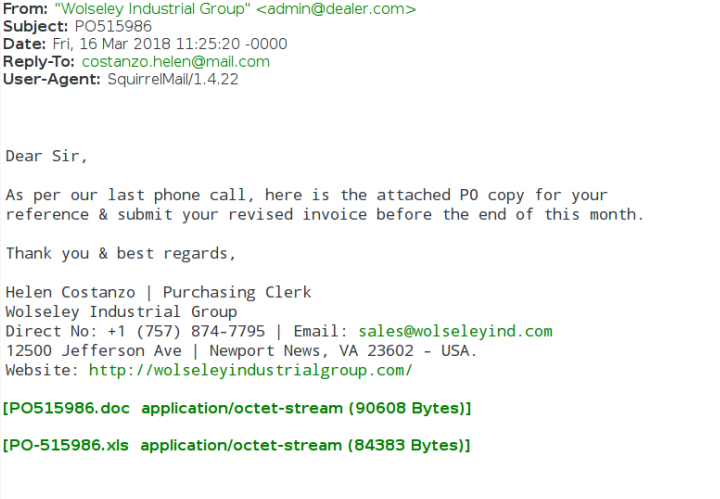
\includegraphics[width=8.45cm]{img/wolseley-industrial-group.png}
	\caption{E-Mail von der Wolseley Industrial Group}
	\label{fig:Wolseley_Industrial_Group}
\end{figure}
Die E-Mail, ersichtlich in Abbildung \ref{fig:Wolseley_Industrial_Group}, erscheint auf den ersten Moment glaubwürdig, denn die Wolseley Industrial Group ist ein in Amerika angesiedeltes Unternehmen und Helen Costanzo ist ein glaubwürdiger Name, vor allem für eine Angestellte eines amerikanischen Unternehmens. Vor allem die Signatur der E-Mail wirkt durch die echten Daten des Unternehmens authentisch. Die Signatur einer E-Mail kann man jedoch heutzutage mit nahezu jedem E-Mail-Programm einfach bearbeiten und somit fälschen. Bei genauerem Hinsehen erkennt man jedoch schnell, dass diese E-Mail gefälscht ist. Als Absender versteckt sich hinter den Namen Wolseley Industrial Group die E-Mail-Adresse \emph{admin@dealer.com}. Diese E-Mail-Adresse taucht auch als Absender anderer dubioser E-Mails auf, unter anderem auch bei einem \glqq Offiziellen Gewinnerbrief\grqq\space einer Lotterie.\cite{gewinnerbrief-admin-dealer} Am 22. März 2018 warnte auch die Wolseley Industrial Group selbst vor gefälschten E-Mails in ihrem Namen.\cite{scam-warnung-wolseley} Das Unternehmen warnt hierbei ausdrücklich davor, die angefügten Dateien zu öffnen, da sie mit Viren belastet sein könnten. Das Unternehmen bezeichnet diese Nachricht hierbei als eine Scam-Mail, also eine E-Mail, in welcher aufgefordert wird einen gewissen Geldbetrag zu bezahlen, um dann zu einem späteren Zeitpunkt daraus irgendeinen materiellen oder finanziellen Gewinn zu erzielen. Der deutsche Fachausdruck hierfür ist \emph{Vorschussbetrug} und ist strafbar.\cite{vorschussbetrug}\\
Welcher Harvester für das Sammeln der E-Mail-Adressen, an welche diese Scamnachrichten geschickt wurden, verantwortlich ist, lässt sich nicht mehr zurückverfolgen. Da zu diesem Zeitpunkt der E-Mail-Adressen-Präfix mit dem Unix-Timestamp, wie unter Punkt \ref{subsub:harverster-tarpit} erwähnt, noch nicht implementiert wurde und ein Harvester diese Adressen zu jedem beliebigen Zeitpunkt X oder gar über mehrere Wochen verteilt gesammelt haben könnte, kann man im Nachhinein nicht mehr zweifelsfrei feststellen, welcher Harvester die betroffenen Adressen eingesammelt hat. Auch das betroffene Unternehmen gibt hierzu keine näheren Auskünfte.
%TODO: EVTL. EINBAUEN
%Ein IP-Lookup\footnote{Bei einem IP-Lookup wird die IP-Adresse zurückverfolgt und man erhält somit Informationen über Besitzer, ungefähren Standort des Endgerätes und vieles mehr.} hat jedoch ergeben, dass die E-Mails von einem Mailserver aus gesendet wurden, welcher in Dallas, Texas steht.
\\Bereits wenige Wochen später, am 12. April 2018, wiederholte sich der zuvor genannte Vorfall: Eine E-Mail, diesmal vom Unternehmen \emph{Bearing Distributors Inc}, fordert den Empfänger auf, die mitgeschickte Rechnung zu überprüfen und an eine Costanzo Helen zurückzuschicken. Das betroffene Unternehmen hat sich bislang (14. April 2018) noch nicht zum Vorfall geäußert.
%TODO: SOGEN DASS LEI E-MAIL ADRESSEN MIT S,A,N,O UNGRBM WORDN SAN UND A POOR NO MIT R UND P
%TODO: DE MARXISMUS-MAIL ERWÄHNEN
	%---Brute-Force-Tarpit---
	\subsubsection{Brute-Force-Tarpit}
Neben der Harvester-Tarpit war auch die Brute-Force-Tarpit erfolgreich. Insgesamt wurden 7.051 Loginversuche getätigt. Hierbei wurden aus zehn verschiedene Benutzernamen und 1.107 verschiedenen Passwörtern 3.793 verschiedene Kombinationen gewählt, somit wurde jede Kombination im Schnitt mehrfach probiert. In den Tabellen \ref{tab:top-ben} und \ref{tab:top-pass} sind die häufigsten Benutzernamen und Passwörter aufgezeigt, welche in der simulierten Wordpressloginform eingegeben wurden.
\begin{table}[htb!]
	\centering
	\begin{tabular}{c|c}
		\textbf{Benutzername}&\textbf{Anzahl an Versuchen}\\\hline
		admin & 2340\\
		maturaprojekt & 1308\\
		test & 1246 \\
		webmaster & 1052\\
		root & 1052 \\
		administrator & 46 \\
	\end{tabular}
	\caption{Die am häufigsten eingegebenen Benutzernamen}
	\label{tab:top-ben}
\end{table}
\begin{table}[htb!]
	\centering
	\begin{tabular}{c|c}
		\textbf{Passwort}&\textbf{Anzahl an Versuchen}\\\hline
		admin & 24\\
		PASSWORD & 24\\
		nicole & 19\\
		michael & 19\\
		daniel & 18\\
		jessica & 17\\
		111111 & 15\\
		lovely & 15\\
		ashley & 15\\
		iloveyou & 14\\
		... & ...\\
		THOMAS & 8\\
	\end{tabular}
	\caption{Die am häufigsten eingegebenen Passwörter}
	\label{tab:top-pass}
\end{table}
\\Analog hierzu sind in Tabelle \ref{tab:top-pass-splash} die zehn häufigsten Passwörter von 2017 aufgezeigt.\footnote{Die zehn häufigsten Passwörter laut SplashData, \href{https://13639-presscdn-0-80-pagely.netdna-ssl.com/wp-content/uploads/2017/12/Top-100-Worst-Passwords-of-2017a.pdf}{hier geht es zur kompletten Liste}.}
\begin{table}[htb!]
	\centering
	\begin{tabular}{c|c}
		\textbf{Platz}&\textbf{Passwort}\\\hline
		1 & 123456\\
		2 & Password\\
		3 & 12345678\\
		4 & qwerty\\
		5 & 12345\\
		6 & 123456789\\
		7 & letmein\\
		8 & 1234567\\
		9 & football\\
		10 & iloveyou\\
	\end{tabular}
	\caption{Die am häufigsten genutzten Passwörter laut SplashData}
	\label{tab:top-pass-splash}
\end{table}
Vergleicht man nun Tabelle \ref{tab:top-pass} mit Tabelle \ref{tab:top-pass-splash}, so kann man deutlich erkennen, dass unter anderem die Standardpasswörter aus Tabelle \ref{tab:top-pass-splash} häufig probiert wurden. Dies lässt sich vor allem dadurch erklären, dass die Betreiber solcher Webcrawler bewusst ihre Liste der zu probierenden Passwörtern mit solchen \glqq typischen Passwörter\grqq\space füllen. Die vielen Vornamen, welche in das Passwortfeld eingetragen wurden, lassen sich jedoch nicht erklären. Wahrscheinlich hat ein Webcrawler eine sogenannte Wörterbuchattacke ausgeführt, sprich er hat Passwörter probiert, welche man in einem Wörterbuch auffinden kann. Hierzu zählen selbstverständlich auch Vornamen. Beeindruckend ist jedoch die Tatsache, dass Webcrawler auch meinen Vornamen als Passwort ausprobiert haben. Meinen Vornamen herauszufinden ist für einen Webcrawler ein leichtes Spiel: Der Meta-Tag \emph{author} in der HTML-Seite enthält den Wert \emph{Thomas Brixen}. Das beeindruckende und zugleich unerklärliche ist jedoch, dass kein einziges mal, weder als Benutzernamen, noch als Passwort, das Wort \emph{Brixen} probiert wurde, obwohl es, wie auch mein Vorname, der Wert des Metatags \emph{author} ist. Selbstverständlich könnte ein Webcrawler den Inhalt des Metatags durch einen Filter laufen lassen und merken, dass \emph{Brixen}, im Gegensatz zu \emph{Thomas}, kein Name ist. Des Weiteren könnte ein Webcrawler auch anhand der IP-Adresse den ungefähren Standort des Webservers zurückverfolgen und würde dann merken, dass \emph{Brixen} eine Stadt im unmittelbaren Umfeld ist. Beides rechtfertigt jedoch nicht, das Wort \emph{Brixen} als einen potentiellen Benutzernamen oder Passwort auszuschließen und deshalb nicht zu probieren.
\begin{table}[htb!]
	\centering
	\begin{tabular}{c|c}
		\textbf{User-Agent (nur Browser)}&\textbf{Anzahl an Loginversuchen}\\\hline
		Firefox/40.1 & 3.755 \\
		Firefox/3.0.15 & 3.152 \\
		\emph{Weitere User-Agents}\footnote{Die restlichen Loginversuche stammen wurden mit verschiedenen User-Agents ausgeführt und sind in ihrer Anzahl so klein, dass sie für die Auswertung nicht relevant sind.} & 144
	\end{tabular}
	\caption{Die User-Agents (nur Browser) mit welchen Loginversuche getätigt wurden}
	\label{tab:top-user-agent}
\end{table}
\\Aus Tabelle \ref{tab:top-user-agent} lässt sich des Weiteren eindeutig erkennen, dass für die Angriffe hauptsächlich zwei Versionen des Browsers Firefox, nämlich die Versionen 40.1 und 3.0.15, verantwortlich waren. Jedoch veröffentlichte Mozilla beispielsweise nie eine Version 40.1 von Firefox.\cite{firefox-versions} Nach kurzer Recherche zeigt sich, dass der User-Agent Firefox/40.1 dafür bekannt ist, weltweit Loginversuche auf Webseiten, welche Wordpress verwenden, zu tätigen.\cite{firefox-40-1} Viele vermuten hinter Firefox/40.1 ein Botnetz\footnote{Ein Botnetz ist eine Ansammlung von Endgeräten, Router, PCs, Smartphones, etc., welche von einem Angreifer aus der Ferne kontrolliert werden können. Durch eine Schadsoftware, welche beispielsweise zuvor über E-Mails verbreitet wurde, werden nach und nach immer mehr Endgeräte in dieses Botnetz aufgenommen. Ein großes Botnetz kann schnell mehrere Tausend Endgeräte umfassen. Meist werden Botnetze für einen DDoS-Angriff verwendet, bei welchem zu einem Zeitpunkt X die infizierten Endgeräte simultan eine Ressource auf einem Webserver anfragen, mit dem Ziel, dass dieser Webserserv die Anfragen nicht stemmen kann und zusammenbricht.}, zu welchem Endgeräte auf der ganzen Welt zusammengeschlossen wurden.\cite{wordpress-botnetz} Diese Vermutung bestätigte sich im Verlaufe dieses Versuches. In der Zeit vom 25. bis zum 28. Februar 2018 wurde VEVETA Opfer eines Angriffes eines Botnetzes. Endgeräte aus 152 verschiedenen Ländern versuchten sich über die Wordpressloginform anzumelden und tappten dabei in die Falle: Die Brute-Force-Tarpit fing sie und loggte ihre Loginversuche mit. Hierbei schienen fast ausschließlich User-Agent mit dem Browser Firefox/40.1 auf. Die Angriffe des Botnetzes kamen hierbei, wie bereits erwähnt, aus 152 verschiedenen Ländern, was in 
%Tabelle \ref{tab:top-countries-botnetz} und 
Abbildung \ref{fig:botnetz-karte} nochmals verdeutlicht wird:\\
%\begin{table}
%	\centering
%	\begin{tabular}{c|c}
%		\textbf{Land}&\textbf{Anzahl der Loginversuch}\\\hline
%		Brasilien & 266\\
%		Indien & 252\\
%		USA & 202\\
%		Philippinen & 167\\
%		Italien & 114\\
%		Malaysia & 102\\
%		Frankreich & 100\\
%		Algerien & 94\\
%		Spanien & 80\\
%		Serbien & 78
%	\end{tabular}
%	\caption{Die Länder, welche während des Angriffes des Botnetzes die meisten Loginversuche tätigten}
%	\label{tab:top-countries-botnetz}
%\end{table}
\begin{figure}[H]
	\centering
	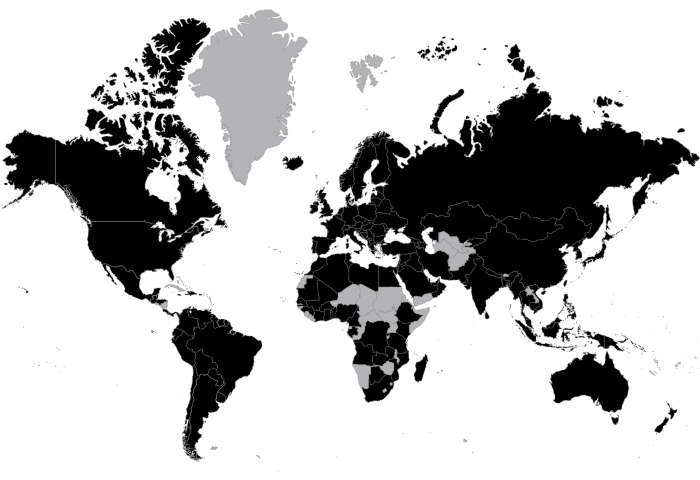
\includegraphics[width=8.45cm]{img/botnetz-angriffe-karte-1920-1080.png}
	\caption{Länder aus denen der Angriff des Botnetzes stammte (schwarz markiert)}
	\label{fig:botnetz-karte}
\end{figure}
Hierbei kann man in Abbildung \ref{fig:botnetz-karte} deutlich erkennen, dass nahezu jedes Land Bestandteil dieses Botnetzes ist. Sowohl  Internetnutzer in Schwellenländern als auch in Industriestaaten wurden Opfer einer schadhaften Software, welche dann später diesen Angriff koordiniert hat.
%TODO:
%\newpage
%EVTL FA DEN ZEUG DO SCHREIBEN
%\begin{table}
%	\centering
%	\begin{tabular}{c|cc}
%		\textbf{Anzahl der Anfragen}&\textbf{Datei}&\textbf{Methode}\\\hline
%		4.574 & / & GET\\
%		3.993 & /wp-login.php & GET\\
%		3.919 & /wp-login.php & POST\\
%		3.782 & /xmlrpc.php & POST\\
%		3.152 & //wp-login.php & POST\\
%		1.862 & - & ---\\
%		1.737 & /wp-admin/ & GET\\
%		1.722 & /test/wp-admin/ & GET\\
%		1.715 & /wordpress/wp-admin/ & GET\\
%		1.712 & /blog/wp-admin/ & GET
%	\end{tabular}
%	\caption{Die am häufigsten angefragten Dateien}
%	\label{tab:top-hits-wordpress}
%\end{table}
	%##########################################
	%---Schlussteil---
	\section{Schlussteil}
	%---Zusammenfassung der Ergebnisse---
	\subsection{Zusammenfassung der Ergebnisse}
	Das Internet als ein immer stärker wachsendes Medium beinhaltet bereits heutzutage eine endlos scheinende Menge an Informationen. Menschen sind mit dieser Fülle an Informationen schon seit langem überfordert. Es wurden Mittel geschaffen diese Menge an Informationen für uns Menschen aufzubereiten, nämlich Webcrawler. Sie sind, auch wenn wir sie kaum bemerken, zu einem der wichtigsten Hilfsmittel in unserer heutigen Onlinewelt geworden. Doch wie so vieles haben auch sie Schattenseiten. Einige Webcrawler versuchen Inhalte von Webseiten zu kopieren, Passwörter zu knacken oder E-Mail-Adressen für einen späteren Versand von Spamnachrichten zu sammeln.\\
Durch einen aggressiven Aufruf von Webseiten versuchen bösartige Webcrawler so schnell als möglich an eine Fülle an Informationen zu gelangen und nehmen dabei auch einen Serverabsturz in Kauf. Regeln der robots.txt werden hierbei bewusst verletzt, ein Serveradministrator ist in solchen Fällen oft machtlos.\\
Das Versenden von Spam- oder Scramnachrichten scheint immer noch ein lukratives Business zu sein. Öffentlich einsehbare E-Mail-Adressen werden gestohlen und landen in den Listen von Harvestern. Es finden sich in den Postfächern der Opfer immer wieder fragwürdige aber echt erscheinende Mails. Diese Mails gehören ohne zu zögern in den Papierkorb, das bloße Öffnen dieser könnte bereits einen Virus starten. Das Imitieren einer E-Mail von einem echten Unternehmen bedeutet auch für dieses einen großen Schaden. Die sinkenden Reputation nach so einem Vorfall ist für ein weltweit operierenden Unternehmen meist der größte finanzielle Schaden, den sie sich vorstellen können.\\
Die in den Mails enthaltenen Viren können unter Umständen auch das betroffene Endgerät übernehmen und in ein Botnetz einhängen. Dieses kann dann mit einem Klick aktiviert werden und von praktisch jedem Land der Welt aus starten Endgeräte DDoS-Attacken oder Brute-Force-Versuche auf Loginformen von populären System, wie etwa Wordpress. Listen von beliebten Kombinationen aus Benutzernamen und Passwörtern werden hier meist über Tage hinweg ausprobiert. Das Opfer ist diesen Angriffen schutzlos ausgeliefert, da die vermeintlichen Angreifer normale Endgeräte sind, welche von unwissenden Nutzern wie Du und Ich verwendet werden und man sie deshalb nicht aussperren kann. Das Opfer kann hierbei nur hoffen, dass seine Kombination aus Benutzernamen und Passwort nicht erraten wird, was bei einem starken Passwort jedoch sehr unwahrscheinlich ist.
	%---Ausblick---
	\subsection{Ausblick}
	Das Durchführen dieses Versuches hat gezeigt, dass unzählige bösartige Webcrawler im Internet ihr Unwesen treiben. Die Zahl von ihnen wird täglich größer. Das Betreiben einer Tarpit als Schutzmaßnahme vor Webcrawlern und ihren Angriffen ist jedoch nicht rentabel. Webcrawler verändern sich über die Zeit, werden schlauer, erkennen Gefahren und reagieren darauf. Um mit den Webcrawlern Schritt halten zu können müssen sich auch die Tarpits dementsprechend weiterentwickeln und hinken dabei den Webcrawlern immer einen Schritt hinterher: Auf ein Angriffsmuster kann erst reagiert werden, nachdem es schon einmal angewendet wurde, doch dann ist es meist schon zu spät.\\
Das Betreiben und Weiterentwickeln von Tarpits ist ein ressourcen- und zeitaufwendiges Unterfangen, dessen Kosten ein Unternehmen erst einmal stemmen muss. Das darin investierte Geld wäre in qualitative Antivirensoftware, Spamfilter oder dergleichen besser investiert. Auch kann eine einzige Tarpit niemals gegen die schier endlose Anzahl an Webcrawlern aufkommen. Fangt man einen, können auf dem Webserver des Betreibers des Webcrawlers noch zehn weitere auf ihren Einsatz warten. Ein Verbund von Tarpits wäre erforderlich, dessen Koordination erneut Unsummen verschlingen würde. Des Weiteren ist zu bedenken, dass sich auch die Betreiber von Webcrawlern zusammenschließen könnten und ein gezielter Angriff von Webcrawlern, welche über ein oder gar mehrere Botnetze betrieben werden, nahezu jeden Webserver in die Knie zwingen könnte.\\
So interessant die Vorstellung einer Tarpit und dessen Konzept der \glqq Rache\grqq\space an einem Webcrawler auch klingt, die Umsetzung ist zum jetzigen Zeitpunkt wirtschaftlich nicht rentabel und praktisch auch nahezu unmöglich. Hier heißt es einfach abwarten was die Zukunft bringt. Doch spätestens dann, wenn die rapiden Fortschritte in der künstlichen Intelligenz Früchte tragen oder die Theorie des Quantencomputers zur Realität wird, müssen wir uns alle Gedanken über unsere Sicherheit im Internet machen, denn unsere jetzigen Sicherheitskonzepte werden bei weitem nicht mehr ausreichend sein.
	\newpage
	\setcounter{page}{1}
	\pagenumbering{Roman}
	\printbibliography
	\listoffigures
	\listoftables
	%\printbibliography[title={Weiterführende Literatur},keyword={further}]
\end{document}

